% Options for packages loaded elsewhere
\PassOptionsToPackage{unicode}{hyperref}
\PassOptionsToPackage{hyphens}{url}
%
\documentclass[
]{book}
\usepackage{amsmath,amssymb,amsfonts,mathabx}
\usepackage{lmodern}
\usepackage{iftex}
\ifPDFTeX
  \usepackage[T1]{fontenc}
  \usepackage[utf8]{inputenc}
  \usepackage{textcomp} % provide euro and other symbols
\else % if luatex or xetex
  %\usepackage{unicode-math}
  %\defaultfontfeatures{Scale=MatchLowercase}
  %\defaultfontfeatures[\rmfamily]{Ligatures=TeX,Scale=1}
%\usepackage{fontspec}
%\setmainfont{Latin Modern Roman}
%\setmathrm{Cambria Math}
\fi
% Use upquote if available, for straight quotes in verbatim environments
\IfFileExists{upquote.sty}{\usepackage{upquote}}{}
\IfFileExists{microtype.sty}{% use microtype if available
  \usepackage[]{microtype}
  \UseMicrotypeSet[protrusion]{basicmath} % disable protrusion for tt fonts
}{}
\makeatletter
\@ifundefined{KOMAClassName}{% if non-KOMA class
  \IfFileExists{parskip.sty}{%
    \usepackage{parskip}
  }{% else
    \setlength{\parindent}{0pt}
    \setlength{\parskip}{6pt plus 2pt minus 1pt}}
}{% if KOMA class
  \KOMAoptions{parskip=half}}
\makeatother
\usepackage{xcolor}
\usepackage{longtable,booktabs,array}
\usepackage{calc} % for calculating minipage widths
% Correct order of tables after \paragraph or \subparagraph
\usepackage{etoolbox}
\makeatletter
\patchcmd\longtable{\par}{\if@noskipsec\mbox{}\fi\par}{}{}
\makeatother
% Allow footnotes in longtable head/foot
\IfFileExists{footnotehyper.sty}{\usepackage{footnotehyper}}{\usepackage{footnote}}
\makesavenoteenv{longtable}
% INSERT PACKAGES
\usepackage{imakeidx}
\makeindex
\usepackage{graphicx}
\usepackage[margin=1in]{geometry}
\usepackage{wrapfig}
\usepackage{graphics}
\usepackage{titling}
\usepackage{fancyhdr}
\pagenumbering{gobble}
\addtocontents{toc}{\protect\thispagestyle{empty}}
\addtocontents{title}{\protect\thispagestyle{empty}}
\setlength{\emergencystretch}{3em} % prevent overfull lines
\providecommand{\tightlist}{%
  \setlength{\itemsep}{0pt}\setlength{\parskip}{0pt}}
\setcounter{secnumdepth}{5}
\usepackage{booktabs}
\usepackage{subfig}
\usepackage{float}
\usepackage{booktabs}
\usepackage{longtable}
\usepackage{array}
\usepackage{multirow}
\usepackage{wrapfig}
\usepackage{float}
\usepackage{colortbl}
\usepackage{pdflscape}
\usepackage{tabu}
\usepackage{threeparttable}
\usepackage{threeparttablex}
\usepackage[normalem]{ulem}
\usepackage{makecell}
\usepackage{xcolor}
\ifLuaTeX
  \usepackage{selnolig}  % disable illegal ligatures
\fi
\usepackage[]{natbib}
\bibliographystyle{plainnat}
\IfFileExists{bookmark.sty}{\usepackage{bookmark}}{\usepackage{hyperref}}
\IfFileExists{xurl.sty}{\usepackage{xurl}}{} % add URL line breaks if available
\urlstyle{same} % disable monospaced font for URLs
\hypersetup{
  pdftitle={Exercises},
  pdfauthor={Joakim Bilyk},
  pdfkeywords={probability theory, insurance mathematics, life insurance,
non-life insurance, stochastic differential equations.},
  hidelinks,
  pdfcreator={LaTeX via pandoc}}

\title{Exercises}
\usepackage{etoolbox}
\makeatletter
\providecommand{\subtitle}[1]{% add subtitle to \maketitle
  \apptocmd{\@title}{\par {\large #1 \par}}{}{}
}
\makeatother
\subtitle{Msc in Actuarial Mathematics}
\author{Joakim Bilyk}
\date{April 08, 2023}

%\usepackage{setspace}\onehalfspacing
%\AtBeginDocument{%
 % \addtolength\abovedisplayskip{0\baselineskip}%
 % \addtolength\belowdisplayskip{0\baselineskip}%
 % \addtolength\abovedisplayshortskip{0\baselineskip}% play with -0.75
 % \addtolength\belowdisplayshortskip{0\baselineskip}%play with -0.5
%}

\begin{document}
\allowdisplaybreaks
\setlength{\abovedisplayskip}{10pt}
\setlength{\belowdisplayskip}{10pt}
\setlength{\abovedisplayshortskip}{-10pt}
\setlength{\belowdisplayshortskip}{0pt}

%\maketitle


{
%title
\begin{titlepage}
\newcommand{\HRule}{\rule{\linewidth}{0.5mm}} % Defines a new command for the horizontal lines, change thickness here

\center % Center everything on the page
 
%----------------------------------------------------------------------------------------
%	HEADING SECTIONS
%----------------------------------------------------------------------------------------

\textsc{\LARGE University of Copenhagen}\\[4cm] % Name of your university/college
\textsc{\Large Msc in Actuarial Mathematics}\\[0.5cm] % Major heading such as course name
%\textsc{\large Assignment 1}\\[0.5cm] % Minor heading such as course title

%----------------------------------------------------------------------------------------
%	TITLE SECTION
%----------------------------------------------------------------------------------------

\HRule \\[0.4cm]
{ \huge \bfseries \thetitle}\\[0.4cm] % Title of your document
\HRule \\[1.5cm]
 
%----------------------------------------------------------------------------------------
%	AUTHOR SECTION
%----------------------------------------------------------------------------------------

\begin{minipage}{0.4\textwidth}
\begin{flushleft} \large
\emph{Author:}\\
\textsc{\theauthor} \\
\end{flushleft}
\end{minipage}
~
\begin{minipage}{0.4\textwidth}
\begin{flushright} \large
\emph{Date:} \\
\textsc{\thedate} \\
\end{flushright}
\end{minipage}\\[2cm]

% If you don't want a supervisor, uncomment the two lines below and remove the section above
%\Large \emph{Author:}\\
%John \textsc{Smith}\\[3cm] % Your name

%----------------------------------------------------------------------------------------
%	DATE SECTION
%----------------------------------------------------------------------------------------

%{\large \thedate}\\[2cm] % Date, change the \today to a set date if you want to be precise

%----------------------------------------------------------------------------------------
%	LOGO SECTION
%----------------------------------------------------------------------------------------


\includegraphics[width = 0.45\textwidth]{logo_ku.png}% Include a department/university logo - this will require the graphicx package
 
%----------------------------------------------------------------------------------------

\vfill % Fill the rest of the page with whitespace
\end{titlepage}

\thispagestyle{empty}
\begin{center}
\textbf{\large Abstract}
\end{center}

This document contain exercises in probability theory and mathematical statistics applied in finance, life insurance and non-life insurance.

Keywords: \emph{probability theory, insurance mathematics, life insurance,
non-life insurance, stochastic differential equations.}
\vfill
\pagebreak

\setcounter{tocdepth}{3}
\tableofcontents
}
\thispagestyle{empty}
\newpage
\setcounter{page}{1}
\pagenumbering{arabic}
\pagestyle{fancy}
\fancyhf{}
\fancyhead[LE]{\fontsize{10}{12} \selectfont\nouppercase{\rightmark\hfill\leftmark}}
\fancyhead[RO]{\fontsize{10}{12} \selectfont\nouppercase{\leftmark\hfill\rightmark}}
\fancyfoot[LE,RO]{\hfill\thepage\hfill}
\hypertarget{introduction}{%
\chapter{Introduction}\label{introduction}}

\hypertarget{abbreviations}{%
\section{Abbreviations}\label{abbreviations}}

Below is given the abbreviations used when referencing to books:

\begin{longtable}[]{@{}
  >{\raggedright\arraybackslash}p{(\columnwidth - 4\tabcolsep) * \real{0.3235}}
  >{\raggedright\arraybackslash}p{(\columnwidth - 4\tabcolsep) * \real{0.1471}}
  >{\raggedright\arraybackslash}p{(\columnwidth - 4\tabcolsep) * \real{0.5294}}@{}}
\toprule()
\begin{minipage}[b]{\linewidth}\raggedright
Chapter
\end{minipage} & \begin{minipage}[b]{\linewidth}\raggedright
Abbreviation
\end{minipage} & \begin{minipage}[b]{\linewidth}\raggedright
Source
\end{minipage} \\
\midrule()
\endhead
Basic Life Insurance Mathematics & & \\
Stochastic Processes in Life Insurance Mathematics & & \\
Life Insurance Mathematics & Asmussen & \emph{Risk and Insurance}: A Graduate Text by Soren Asmussen and Mogens Steffensen (2020). \\
& Bladt & Notes from lectures in Liv2. \\
Topics in Life Insurance Mathematics & Asmussen & \emph{Risk and Insurance}: A Graduate Text by Soren Asmussen and Mogens Steffensen (2020). \\
Continuous Time Finance & Bjork & \emph{Arbitrage Theory in Continuous Time (Fourth edition)} by Thomas Bjork, Oxford University Press (2019). \\
Basic Non-Life Insurance Mathematics & & \\
Stochastic Processes in Life Insurance Mathematics & & \\
Topics in Non-Life Insurance Mathematics & & \\
Probabilistic Machine Learning & \emph{None} & Slides from lectures. \\
Quantative Risk Management & & \\
Measure Theory & Bjork & \emph{Arbitrage Theory in Continuous Time (Fourth edition)} by Thomas Bjork, Oxford University Press (2019). \\
& Protter & \emph{Probability Essentials (2. edition)} by Jean Jacod and Philip Protter (2004). \\
Random Variables & Bjork & \emph{Arbitrage Theory in Continuous Time (Fourth edition)} by Thomas Bjork, Oxford University Press (2019). \\
& Hansen & \emph{Stochastic Processes} (2. edition) by Ernst Hansen (2021). \\
Discrete Time Stochastic Processes & Hansen & \emph{Stochastic Processes} (2. edition) by Ernst Hansen (2021). \\
Continuous Time Stochastic Processes & Bjork & \emph{Arbitrage Theory in Continuous Time (Fourth edition)} by Thomas Bjork, Oxford University Press (2019). \\
Stochastic Calculus & Bjork & \emph{Arbitrage Theory in Continuous Time (Fourth edition)} by Thomas Bjork, Oxford University Press (2019). \\
& Bladt & Notes from lectures in Liv2. \\
Linear Algebra & Wiki & Wikipedia \\
\bottomrule()
\end{longtable}

\hypertarget{to-do-work}{%
\section{To-do work}\label{to-do-work}}

\begin{longtable}[]{@{}lll@{}}
\toprule()
Chapter & Note & Progress \\
\midrule()
\endhead
ML & Exercises week 1 & \\
\bottomrule()
\end{longtable}

\hypertarget{continuous-time-finance}{%
\chapter{Continuous Time Finance}\label{continuous-time-finance}}

\hypertarget{week-1}{%
\section{Week 1}\label{week-1}}

\textbf{Probability exercises}

Let \((W(t))_{t\ge}\) be a Brownian motion (Bjork, Definition 4.1).

\textbf{Exercise 1.} Show that the following processes also are Brownian motions.

\begin{enumerate}
\def\labelenumi{\roman{enumi}.}
\tightlist
\item
  \((-W(t))_{t\ge 0}\) (symmetry)
\item
  For any \(s\ge 0\), \((W(t+s)-W(s))_{t\ge 0}\) (time-homogeneity).
\item
  For every \(c>0\), \((cW(t/c^2))_{t\ge 0}\) (scaling).
\end{enumerate}

\textbf{Solution (i).}

By assumption \(W\) is a Brownian motion and so it follows that

\[-W_0=-1\cdot0=0\]

Furthermore, for \(r<s\le t< u\) it holds that \(W_u-W_t\) and \(W_s-W_r\) is independent. By seperate transformations the independence property is preserved and \(-(W_u-W_t)\) and \(-(W_s-W_r)\) is independent. Next, for a normal distributed random variable \(N\sim\mathcal{N}(\mu,\sigma^2)\) it holds, that for a scaler \(c\in\mathbb{R}\) we have \(c N\sim\mathcal{N}(c\mu,c^2\sigma ^2)\). Then obviously;

\[-(W_t)=(-1)W_t\stackrel{d}{=}\mathcal{N}((-1)\cdot0,(-1)^2(t-s))\stackrel{d}{=}\mathcal{N}( 0,t-s).\]

Lastly, let \(\omega \in \Omega\) and consider the sample path \(s\mapsto (-W_s)(\omega)\). Clearly for two continuous functions \(f\) and \(g\) it holds that \((g\circ f)\) is continuous. Then with \(g(f)=-f\) and \(f(t)=W_t(\omega)"/>\) it follows that \((-W_t)=(g\circ W)(t)\) is also continuous.

\textbf{Solution (ii).}

Much like the previous exercise we define a new process and show the properties hold. Let \(s\ge 0\) be chosen arbitrary. Now define \(X_t=W(t+s)-W(s)\).

First, we let \(t=0\) and see

\[X_0=W(0+s)-W(s)=W(s)-W(s)=0.\]

Secondly, we have that for \(r<u\):

\[X_u-X_r=W(u+s)-W(s)-(W(r+s)-W(s))=W(u+s)-W(r+s)\sim \mathcal{N}(0,u+s-(r+s))=\mathcal{N}(0,u-r).\]

and since for \(r<u\le k<l\) the translation \(r+s<u+s\le k+s<l+s\) still holds and \(X_l-X_k=W(l+s)-W(k+s)\) and \(X_u-X_r=W(u+s)-W(k+s)\) are independent. Finally since \(W_t(\omega)\) is continuous in \(t\) hence the translation \(W_{t+s}\) is continouos. Adding a constant yields a function that is also continuous, hence \(X_t\) is continuous.

\textbf{Solution (iii).}

Let \(c>0\) be given. We show that

\[X_t=cW\left(\frac{t}{c^2}\right)\]

is a Brownian motion. We simply show the four properties. Let \(t=0\) and notice

\[X_0=cW\left(\frac{0}{c^2}\right)=cW(0)=0.\]

The second property follows from seperate transformation and that for \(r<u\le s<t\) we consider

\[X_u-X_r=c\left(W\left(\frac{u}{c^2}\right)-W\left(\frac{r}{c^2}\right)\right)\hspace{20pt}\text{and}\hspace{20pt}X_t-X_s=c\left(W\left(\frac{t}{c^2}\right)-W\left(\frac{s}{c^2}\right)\right)\]

and since \(c,r,u,t,s>0\) we have the same order for the scaled version of \(r,u,t,s\) and hence we have two independent RV scaled by \(c\). Then by seperate transformations the variables is still independent. Next for the third property:

\[X_t-X_s=c\left(W\left(\frac{t}{c^2}\right)-W\left(\frac{s}{c^2}\right)\right)\sim\mathcal{N}\left(c\cdot 0,c^2\left(\frac{t}{c^2}-\frac{s}{c^2}\right)\right)=\mathcal{N}(0,t-s).\]

Where we use the properties of scaling a normal distributed random variable i.e.~for \(c>0\) and \(N\sim\mathcal{N}(\mu,\sigma ^2)\) it follows that \(c N\sim\mathcal{N}(c\mu,c^2\sigma ^2)\). Finally, the forth property follows since \(g(f)=cf\) is continuous and \(h(t)=t/c^2\) is continuous, then for any continuous function \(f(s)\) it follows that \((g \circ f\circ h)=g(f(h(t)))\) is continuous.

~

\textbf{Proposition B.37.} Let \((\Omega,\mathcal{F},P)\) be a given probability space, let \(\mathcal{G}\) be a sub-sigma-algebra of \(\mathcal{F}\), and let \(X\) be a square integrable random variable.
Consider the problem of minimizing
\[E\left[(X-Z)^2\right]\]
where \(Z\) is allowed to vary over the class of all square integrable \(\mathcal{G}\) measurable random variables. The optimal solution \(\hat{Z}\) is then given by.
\[\hat{Z}=E[X\vert\mathcal{G}].\]

\textbf{Exercise 2.} \emph{(Bjork, exercise B.11.)} Prove proposition B.37 by going along the following lines.

\begin{enumerate}
\def\labelenumi{\alph{enumi}.}
\tightlist
\item
  Prove that the ``estimation error'' \(X-E[X\vert\mathcal{G}]\) is orthogonal to \(L^2(\Omega,\mathcal{G},P)\) in the sence that for any \(Z\in L^2(\Omega,\mathcal{G},P)\) we have
  \[E[Z\cdot(X-E[X\vert\mathcal{G}])]=0\]
\item
  Now prove the proposition by writing
  \[X-Z=(X-E[X\vert\mathcal{G}])+(E[X\vert\mathcal{G}]-Z)\]
  and use the result just proved.
\end{enumerate}

\textbf{Solution (a).}

Let \(X\in L^2(\Omega,\mathcal{F},P)\) be a random variable. Now consider an arbitrary \(Z\in L^2(\Omega,\mathcal{G},P)\). Recall that \(\mathcal{G}\subset \mathcal{F}\) and so \(X\) is also in \(Z\in L^2(\Omega,\mathcal{G},P)\), as it is bothe square integrable and \(\mathcal{G}\)-measurable. Then

\[E\left[Z\cdot(X-E[X\vert\mathcal{G}])\right]=E\left[Z\cdot X\right]-E\left[Z\cdot E[X\vert\mathcal{G}]\right].\]

Then by using the law of total expectation and secondly that \(Z\) is \(\mathcal{G}\)-measurable we have that

\[E\left[Z\cdot X\right]=E\left[E[Z\cdot X\vert\mathcal{G}]\right]=E\left[Z\cdot E[ X\vert\mathcal{G}]\right].\]

Combining the two equations gives the desired result.

\textbf{Solution (b).}

Obviously, we have that

\[X-Z=X-Z+E[X\vert\mathcal{G}]-E[X\vert\mathcal{G}]=(X-E[X\vert\mathcal{G}])+(E[X\vert\mathcal{G}]-Z).\]

Then squaring the terms gives

\[(X-Z)^2=(X-E[X\vert\mathcal{G}])^2+(E[X\vert\mathcal{G}]-Z)^2+2(X-E[X\vert\mathcal{G}])(E[X\vert\mathcal{G}]-Z)\]

Taking expectation on each side and using linearity of the expectation we have that

\[E[(X-Z)^2]=E\left[(X-E[X\vert\mathcal{G}])^2\right]+E\left[(E[X\vert\mathcal{G}]-Z)^2\right]+2E\left[(X-E[X\vert\mathcal{G}])(E[X\vert\mathcal{G}]-Z)\right].\]

We can now use that \(E[X\vert\mathcal{G}]-Z\) is \(\mathcal{G}\)-measurable with the above result on the last term.

\[E[(X-Z)^2]=E\left[(X-E[X\vert\mathcal{G}])^2\right]+E\left[(E[X\vert\mathcal{G}]-Z)^2\right].\]

Now since \(X\) is given the term \(E\left[(X-E[X\vert\mathcal{G}])^2\right]\) is simply a constant not depending on the choice og \(Z\). The optimal choice of \(Z\) is then \(E[X\vert\mathcal{G}]\) since this minimizes the second term. The statement is then proved.

~

\textbf{Exercise 3.} Discuss the following theory/results of Moment generating functions (Laplace transform).

Let \(X\) be a random variable with distribution function \(F(x)=P(X\le x)\) and \(Y\) be a random variable with distribution function \(G(y)=P(Y\le y)\).

\textbf{Definition.} The moment generating function or Laplace transform of \(X\) is

\[\psi_X(\lambda)=E\left[e^{\lambda X}\right]=\int_{-\infty}^\infty e^{\lambda x}dF(x)\]

provided the expectation is finite for \(\vert\lambda\vert<h\) for some \(h>0\).

The MGF uniquely determine the distribution of a random variable, due to the following result.

\textbf{Theorem 1.} \emph{(Uniqueness)} If \(\psi_X(\lambda)=\psi_Y(\lambda)\) when \(\vert\lambda\vert<h\) for some \(h>0\), then \(X\) and \(Y\) has the same distribution, that is, \(F=G\).

There is also the following result of independence for Moment generating functions.

\textbf{Theorem 1.} \emph{(Independence)} If

\[E\left[e^{\lambda_1X+\lambda_2Y}\right]=\psi_X(\lambda_1)\psi_Y(\lambda_2)\]

for \(\vert\lambda_i\vert<h\) for \(i=1,2\) for some \(h>0\), then \(X\) and \(Y\) are independent random variables.

\textbf{Example.} Recall that the Moment generating function of a normal (Gaussian) distribution is given by

\[\psi_X(\lambda)=E\left[e^{\lambda X}\right]=\exp\left(\lambda \mu + \frac{\lambda^2}{2}\sigma^2\right)\]

where \(X\) is normally distributed with mean \(\mu\) and variance \(\sigma^2\) and \(\lambda\in\mathbb{R}\) is a constant. Since a Brownian motion \(W(t)\) is normally distributed with zero mean and variance \(t\), we have that

\[E[\exp(\lambda W(t))]=\exp\left(\frac{\lambda^2}{2}t\right).\]

\textbf{Discussion.}

~

\textbf{Exercise 4.} \emph{(Bjork, exercise C.8.(a-c))} Let \(W\) be a Brownian motion. Notice that for the natural filtration \(\mathcal{F}_s=\sigma(W_t\vert t\le s)\) \(W_t-W_s\) is independent of \(\mathcal{F}_s\)

\begin{enumerate}
\def\labelenumi{\alph{enumi}.}
\tightlist
\item
  Show that \(W_t\) is a martingale.
\item
  Show that \(W^2_t-t\) is a martingale.
\item
  Show that \(\exp(\lambda W_t-\frac{\lambda^2}{2}t)\) is a martingale.
\end{enumerate}

\textbf{Solution (a).}

We show that for the natural filtration that \(W_t\) is a martingale. This include showing integrability and the martingale property. For the first we note that for a normal distributed random variable with mean 0 we have

\[E[\vert N\vert]=\int_{-\infty}^\infty \vert x\vert dF_N(x)=2\int_{0}^\infty xdF_N(x)\]

since the distribution is symmetric. Substituting the distribution function \(\Phi(x)=P(N\le x)\) in we see that

\[E[\vert N\vert]=2\int_{0}^\infty xd\Phi(x)=2\int_{0}^\infty x\frac{1}{\sqrt{2\pi\sigma^2}}e^{-x^2/(2\sigma^2)}dx=(*)\]

by substituting \(u=x^2/(2\sigma^2)\) (\(x=\sqrt{2\sigma^2u}\)) we have that

\[\frac{dx}{du}=\frac{1}{2}\sqrt{2\sigma^2u}2\sigma^2=(\sigma^2)^{3/2}\sqrt{2}u\iff dx=(\sigma^2)^{3/2}\sqrt{2}u\ du\]

hence

\[(*)=\frac{2}{\sqrt{2\pi\sigma^2}}\int_0^{\infty}\sqrt{2\sigma^2u}e^{-u}(\sigma^2)^{3/2}\sqrt{2}u\ du=\frac{2\sqrt{2\sigma^2}(\sigma^2)^{3/2}\sqrt{2}}{\sqrt{2\pi\sigma^2}}\int_0^{\infty}\sqrt{u}e^{-u}u\ du.\]

This then simplify to

\[(*)=\frac{(2\sigma^2)^{3/2}}{\sqrt{\pi}}\int_0^{\infty}u^{3/2}e^{-u}\ du=(2\sigma^2)^{1/2}\sqrt{\frac{2\sigma^2}{\pi}}\int_0^{\infty}u^{3/2}e^{-u}\ du=\sqrt{\frac{2\sigma^2}{\pi}}<\infty.\]

(Obviously the above is not derived correctly, but the end expression is valid, source: \href{https://arxiv.org/pdf/1402.3559.pdf}{link}) However since

\[W_t=W_t-0=W_t-W_0\sim\mathcal{N}(0,t)\]

we have that \(E\vert W_t\vert<\infty\) as desired.

Next, we have that

\[E[W_t\vert \mathcal{F}_s]=E[W_t-W_s\vert\mathcal{F}_s]+W_s=0+W_s=W_s.\]

In the above we used that \(W_t-W_s\) is \(\mathcal{F}_s\)-measurable with mean 0. Then it follows that \(W_t\) is a martingale.

\textbf{Solution (b).}

Let \(M_t=W_t^2-t\). First, we observe that two measurable functions composed is still a measurable function. Hence we know that \(M_t\) is measurable wrt. the filtration since \(W_t\) is measurable and \(w\mapsto w^2+t\) is measurable. Secondly, we have that

\[E[\vert W_t^2-t\vert]\le E\vert W_t^2\vert +E\vert t\vert=t+t=2t<\infty\]

where we use the triangle inequality. Thirdly, for the martingale property we have that for \(t>s\):

\[E[M_t\vert \mathcal{F}_s]=E[W_t^2-t\vert \mathcal{F}_s]=E[W_t^2+W_s^2-2W_tW_s-W_s^2+2W_tW_s-t\vert \mathcal{F}_s]\]

which by linearity and independence of increments to the filtration gives

\[E[M_t\vert \mathcal{F}_s]=E[(W_t-W_s)^2-W_s^2+2W_tW_s-t\vert \mathcal{F}_s]=t-s-t+E[2W_tW_s-W_s^2\vert \mathcal{F}_s]\]

However since \(W_s\) is measurable wrt. the filtration at time \(s\) the above is

\[E[M_t\vert \mathcal{F}_s]=2W_sE[W_t\vert \mathcal{F}_s]-W_s^2-s=2W_s^2-W_s^2-s=W_s^2-s=M_s.\]

Since from (a) we know that \(W_t\) is a martingale. Then we arrive at the desired result.

\textbf{Solution (c).}

Let \(M_t=\exp\left(\lambda W_t-\frac{\lambda^2}{2}t\right)\). First, by composition of measurable functions \(M_t\) is \(\mathcal{F}_t\)-measurable. Secondly, we have using the MGF for a normal distributed random variable:

\[E\vert M_t=E\left(\exp\left(\lambda W_t-\frac{\lambda^2}{2}t\right)\right)\le E\left(\exp\left(\lambda W_t\right)\right)=\exp\left(\frac{\lambda^2}{2}t\right)<\infty.\]

Thirdly, we consider

\[E[M_t\vert\mathcal{F}_s]=E\left.\left[\left(\exp\left(\lambda W_t-\frac{\lambda^2}{2}t\right)\right)\right\vert\mathcal{F}_s\right]=\exp\left(-\frac{\lambda^2}{2}t\right)E\left.\left[\left(\exp\left(\lambda W_t\right)\right)\right\vert\mathcal{F}_s\right].\]

By adding and subtracting \(W_s\) in the exponent we get

\begin{align*}
E[M_t\vert\mathcal{F}_s]&=\exp\left(-\frac{\lambda^2}{2}t\right)E\left.\left[\left(\exp\left(\lambda (W_t-W_s)+\lambda W_s\right)\right)\right\vert\mathcal{F}_s\right]\\
&=\exp\left(-\frac{\lambda^2}{2}t\right)\exp\left(\frac{\lambda^2}{2}(t-s)\right)E\left.\left[\left(\exp\left(\lambda W_s\right)\right)\right\vert\mathcal{F}_s\right].
\end{align*}

Using that \(E\left.\left[\left(\exp\left(\lambda W_s\right)\right)\right\vert\mathcal{F}_s\right]=\exp\left(\lambda W_s\right)\) and combining the exponents gives the desired:

\[E[M_t\vert\mathcal{F}_s]=\exp\left(\lambda W_s-\frac{\lambda^2}{2}s\right)=M_s.\]

\hypertarget{week-2}{%
\section{Week 2}\label{week-2}}

\textbf{Exercise 1} \emph{(Bjork 4.1)} Compute the stochastic differential \(dZ_t\) when

\begin{enumerate}
\def\labelenumi{\alph{enumi}.}
\tightlist
\item
  \(Z_t=e^{\alpha t}\).
\item
  \(Z_t=\int_0^t g_s\ dW_s\), where \(g\) is an adapted stochastic process.
\item
  \(Z_t=e^{\alpha W_t}\).
\item
  \(Z_t=e^{\alpha X_t}\), where \(X\) has stochastic differential \(dX_t=\mu\ dt + \sigma\ dW_t\) and \(\mu,\sigma\) is constants.
\item
  \(Z_t=X_t^2\), where \(X\) has stochastic differential \(dX_t=\alpha X_t\ dt+\sigma X_t\ dW_t\).
\end{enumerate}

\textbf{Solution (a).}

Let \(Z_t=e^{\alpha t}\), then we see that \(f(t,x)=e^{\alpha t}\) and the the following relevant derivatives is

\[
\frac{\partial f}{\partial t}(t,x)=\alpha e^{\alpha t},\hspace{10pt}\frac{\partial f}{\partial x}(t,x) =0,\hspace{10pt}\frac{\partial f}{\partial x^2}(t,x) =0.
\]

Since \(Z\) does not depend on any stochastic process, we will content with \(X_t=0\), that is \(\mu_t=\sigma_t=0\). Then by theorem 4.11 (Ito's formula) we have

\[
dZ_t=\left(\alpha e^{\alpha t} +0+0\right)\ dt + 0=\alpha e^{\alpha t}\ dt,
\]

as expected. \(\square\)

\textbf{Solution (b).}

Let \(Z_t=\int_0^t g_s\ dW_s\), where \(g\) is an adapted stochastic process. We see that if we set \(X_t=\int_0^t g_s\ dW_s\) then

\[
dX_t=0\ dt+g_t\ dW_t.
\]

Then we have the function \(f(t,x)=x\) and the relevant derivatives are:

\[
\frac{\partial f}{\partial t}(t,x)=0,\hspace{10pt}\frac{\partial f}{\partial x}(t,x) =1,\hspace{10pt}\frac{\partial f}{\partial x^2}(t,x) =0.
\]

This then gives

\[
dZ_t=\left(0+0+\frac{1}{2}g_t\cdot 0\right)\ dt + g_t\cdot 1\ dW_t=g_t\ dW_t,
\]

as expected. \(\square\)

\textbf{Solution (c).}

Let \(Z_t=e^{\alpha W_t}\). Then we may set \(X_t=W_t\) and we then have \(\mu_t=0\) and \(\sigma_t=1\). The function \(f(t,x)=e^{\alpha x}\) and the relevant derivatives are:

\[
\frac{\partial f}{\partial t}(t,x)=0,\hspace{10pt}\frac{\partial f}{\partial x}(t,x) =\alpha e^{\alpha x},\hspace{10pt}\frac{\partial f}{\partial x^2}(t,x) =\alpha^2 e^{\alpha x}.
\]

Then the dynamics of \(Z_t\) is as follows

\begin{align*}
dZ_t&=\left(0+0+\frac{1}{2}1^2\alpha^2e^{\alpha X_t}\right)\ dt + 1\alpha e^{\alpha X_t}\ dW_t\\
&=\frac{\alpha^2}{2}e^{\alpha X_t}\ dt +\alpha e^{\alpha X_t}\ dW_t\\
&=\frac{\alpha^2}{2}Z_t\ dt +\alpha Z_t\ dW_t.
\end{align*}

As desired. \(\square\).

\textbf{Solution (d).}

Let \(Z_t=e^{\alpha X_t}\), where \(X\) has stochastic differential \(dX_t=\mu\ dt + \sigma\ dW_t\) and \(\mu,\sigma\) is constants. Then we have been given the definition of \(X_t\) and we set \(f(t,x)=e^{\alpha x}\). The relevant derivatives are then:

\[
\frac{\partial f}{\partial t}(t,x)=0,\hspace{10pt}\frac{\partial f}{\partial x}(t,x) =\alpha e^{\alpha x},\hspace{10pt}\frac{\partial f}{\partial x^2}(t,x) =\alpha^2 e^{\alpha x}.
\]

We may now derive the dynamics of \(Z_t\):

\begin{align*}
dZ_t&=\left(0+\mu \alpha e^{\alpha X_t}+\frac{1}{2} \sigma^2\alpha^2 e^{\alpha X_t}\right)\ dt+\sigma \alpha e^{\alpha X_t}\ dW_t\\
&=\left(\mu+\frac{1}{2}\sigma^2\alpha\right)\alpha e^{\alpha X_t}\ dt+\sigma \alpha e^{\alpha X_t}\ dW_t\\
&=\left(\mu+\frac{1}{2}\sigma^2\alpha\right)\alpha Z_t\ dt+\sigma \alpha Z_t\ dW_t.
\end{align*}

As desired. \(\square\).

\textbf{Solution (e).}

Let \(Z_t=X_t^2\), where \(X\) has stochastic differential \(dX_t=\alpha X_t\ dt+\sigma X_t\ dW_t\). Then we set \(f(t,x)=x^2\) and the relevant derivatives are:

\[
\frac{\partial f}{\partial t}(t,x)=0,\hspace{10pt}\frac{\partial f}{\partial x}(t,x) =2x,\hspace{10pt}\frac{\partial f}{\partial x^2}(t,x) =2.
\]

Given this we have the dynamics of \(Z_t\) as follows

\begin{align*}
dZ_t&=\left(0 + \alpha X_t2X_t+\frac{1}{2}(\sigma X_t)^22\right)\ dt+\sigma X_t 2 X_t\ dW_t\\
&=\left(2\alpha +\sigma^2\right) X_t^2\ dt + 2\sigma X_t^2\ dW_t\\
&=\left(2\alpha +\sigma^2\right) Z_t\ dt + 2\sigma Z_t\ dW_t.
\end{align*}

As desired. \(\square\).

\textbf{Exercise 2} \emph{(Bjork 4.2)} Compute the stochastic differential for \(Z\) when \(Z_t=(X_t)^{-1}\) and \(X\) has the stochastic differential

\[
dX_t=\alpha X_t\ dt + \sigma X_t\ dW_t.
\]

Furthermore, by using the definition \(Z=X^{-1}\) you can in fact express the right-hand side of \(dZ\) entirely in terms of \(Z\) itself (rather then in terms of \(X\)). Thus \(Z\) satisfies a stochastic differential equation. Which one?

\textbf{Solution.}

We see that \(f(t,x)=1/x\) and so the relevant derivatives is

\[
\frac{\partial f}{\partial t}(t,x)=0,\hspace{10pt}\frac{\partial f}{\partial x}(t,x) =-\frac{1}{x^2},\hspace{10pt}\frac{\partial f}{\partial x^2}(t,x) =\frac{2}{x^3}.
\]

Then we by Ito's formula we have

\begin{align*}
dZ_t&=\left(0-\alpha X_t\frac{1}{X_t^2}+\frac{1}{2} \sigma^2 X_t^2\frac{2}{X_t^3}\right)\ dt-\sigma X_t\frac{1}{X_t^2}\ dW_t\\
&=\left(-\alpha \frac{1}{X_t}+ \sigma^2 \frac{1}{X_t}\right)\ dt-\sigma \frac{1}{X_t}\ dW_t\\
&=(\sigma^2-\alpha)Z_t\ dt-\sigma Z_t\ dW_t.
\end{align*}

We also notice that

\[
Z_t=\frac{1}{X_t}\Rightarrow dZ_t=d\left(\frac{1}{X_t}\right)=-\left(\frac{1}{X_t}\right)^2\ dX_t=-Z_t^2(\alpha X_t\ dt+\sigma X_t\ dW_t)
\]

Hence we may insert \(X_t=Z_t^{-1}\) and optain

\[
dZ_t=-Z_t^2\left(\alpha\frac{1}{Z_t}\ dt + \sigma \frac{1}{Z_t}\ dW_t\right)=-\alpha Z_t\ dt-\sigma Z_t\ dW_t.
\]

Which clearly is faulty.. \(\square\)

\textbf{Exercise 3.} \emph{(Bjork 4.3)} Let \(\sigma(t)\) be a given deterministic function of time and define the process \(X\) by

\[
X_t=\int_0^t\sigma(s)\ dW_s.
\]

Use the technique discribed in example 4.17 in order to show that the characteristic function of \(X_t\) (for a fixed \(t\)) is given by

\[
E[e^{iuX_t}]=\exp\left\{-\frac{u^2}{2}\int_0^t\sigma^2(s)\ ds\right\},\ \ u\in\mathbb{R},
\]

thus showing that \(X_t\) is normally distributed with zero mean and a variance given by

\[
Var[X_t]=\int_0^t\sigma^2(s)\ ds.
\]

\textbf{Solution.}

We follow along the lines of

\begin{enumerate}
\def\labelenumi{\arabic{enumi}.}
\tightlist
\item
  Determine the dynamics of \(Z_t=e^{iuX_t}\) (for fixed \(u\)).
\item
  Write the integral form of \(Z_t\).
\item
  Take expectation.
\item
  Solve ODE.
\end{enumerate}

``1)'' Set \(f(t,x)=e^{iuX_t}\) then the relevant derivatives are

\[
\frac{\partial f}{\partial t}(t,x)=0,\hspace{10pt}\frac{\partial f}{\partial x}(t,x) =iue^{iuX_t}=iuZ_t,\hspace{10pt}\frac{\partial f}{\partial x^2}(t,x) =i^2u^2e^{iuX_t}=-u^2Z_t.
\]

Recall that \(dX_t=\sigma(t)\ dW_t\), then by Ito's formula we have

\[
dZ_t=\left(-\sigma(t)^2\frac{1}{2}u^2Z_t\right)\ dt+\sigma(t)iuZ_t\ dW_t.\tag{*}
\]

``2)'' We can now write (*) on integral form as below

\[
Z_t=Z_0-\frac{u^2}{2}\int_0^t\sigma^2(s)Z_s\ ds+iu\int_0^t\sigma (s)Z_s\ dW_s,
\]

where \(Z_0=e^{iuX_0}=1\).

``3)'' Taking expectation now yields

\[
E[Z_t]=1-\frac{u^2}{2}\int_0^t\sigma^2(s)E[Z_s]\ ds+iuE\left[\int_0^t \sigma(s)Z_s\ dW_s\right]=1-\frac{u^2}{2}\int_0^t\sigma^2(s)E[Z_s]\ ds,
\]

since any expectaion of an integral wrt. a Brownian motion is 0 (proposition 4.5).

``4)'' Now we see that the \(t\)-derivative gives

\[
dE[Z_t]=-\frac{u^2}{2}\sigma^2(t)E[Z_t]\ dt,\ \ E[Z_0]=1.
\]

This is a ordinary differential equation with solution \(y(t)=\exp\{-u^2/2\int_0^t\sigma^2(s)\ ds\}\) (check by differentiating) hence

\[
E[e^{iuX_t}]=E[Z_t]=\exp\left\{-\frac{u^2}{2}\int_0^t\sigma^2(s)\ ds\right\}.
\]

We recognize this as the characteristic function of a normally distributed random variable with variance \(\int_0^t\sigma^2(s)\ ds\) as desired. (\(X_t\) follows this distributions since characteristic functions determine the distribution) \(\square\)

\textbf{Exercise 4} \emph{(Bjork 4.4)} Suppose that \(X\) has the stochastic differential

\[
dX_t=\alpha X_t\ dt+\sigma_t\ dW_t,
\]

where \(\alpha\) is a real number and \(\sigma_t\) is a integrable adapted stochastic process. Use the technique in example 4.17 in order to determine the function \(m(t)=E[X_t]\).

\textbf{Solution.}

We follow the same steps as the previous exercise. We have been given the dynamics of \(X\) hence we may write it on integral form.

\[
X_t=X_0+\alpha\int_0^tX_s\ ds+\int_0^t\sigma(s)\ dW_s.
\]

Then taking expectation now gives

\[
E[X_t]=X_0+\alpha\int_0^tE[X_s]\ ds.
\]

Hence \(E[X_t]\) follows from the solution to the ODE below

\[
dE[X_t]=\alpha E[X_t]\Rightarrow E[X_t]=C\cdot\exp\{\alpha t\}.
\]

Then obviously \(C=X_0\) and we arrive at the solution \(E[X_t]=X_0e^{\alpha t}\), where \(X_0\) is some deterministic value. \(\square\)

\textbf{Exercise 5} \emph{(Bjork 4.5)} Suppose that the process \(X\) has a stochastic differential

\[
dX_t=\mu_t\ dt+\sigma_t\ dW_t,
\]

and that \(\mu_t\ge 0\) with probability one for all \(t\ge 0\). Show that this implies that \(X\) is a sub-martingale.

\textbf{Solution.}

Note that we are (strictly speaking) supposed to show adaptation and integrability, we will however only fokus on the submartingale property.

``\(E[X_t\vert \mathcal{F}_s]\ge X_s\)'' Intuitively speaking, the statement is obvious since we have with probability one a positive upwards drift with Brownian distortion (i.e.~martingale). Formally, we will show the statement by first writing \(X_t\) on integral form

\[
X_t=x_0+\int_0^t\mu_s\ ds+\int_0^t\sigma_s\ dW_s.
\]

And so

\[
X_t-X_s=\int_s^t\mu_u\ du+\int_s^t\sigma_u\ dW_u.
\]

We then have

\begin{align*}
E[X_t\ \vert\ \mathcal{F}_s]-X_s&=E[X_t-X_s\ \vert\ \mathcal{F}_s]\\
&=E\left[\left.\int_s^t\mu_u\ du+\int_s^t\sigma_u\ dW_u\ \right\vert\ \mathcal{F}_s\right]\\
&=E\left[\left.\int_s^t\mu_u\ du\ \right\vert\ \mathcal{F}_s\right]+E\left[\left.\int_s^t\sigma_u\ dW_u\ \right\vert\ \mathcal{F}_s\right]\\
&=E\left[\left.\int_s^t\mu_u\ du\ \right\vert\ \mathcal{F}_s\right]\ge 0.
\end{align*}

Then adding \(X_s\) to the above inequality yields the result. \(\square\)

\textbf{Exercise 6} \emph{(Bjork 4.7)} The objective of this exercise is to give an argument for the formal identity

\[
dW_1(t)\cdot dW_2(t)=0,
\]

when \(W_1\) and \(W_2\) are independent Brownian motions. Let us therefore fix a time \(t\), and divide the inerval \([0,t]\) into equidistant points \(0=t_0<t_1<\cdots < t_n=t\), where \(t_i=\frac{i}{n}\cdot t\). We use the notation

\[
\Delta W_i(t_k)=W_i(t_k)-W_i(t_{k-1}),\ i=1,2.
\]

Now define \(Q_n\) by

\[
Q_n=\sum_{k=1}^n \Delta W_1(t_k)\cdot \Delta W_2(t_k).
\]

Show that \(Q_n\to 0\) in \(L^2\), i.e.~show that

\[
E[Q_n]=0,\\
Var[Q_n]\to 0.
\]

\textbf{Solution.}

We wish to show the statement

\[
E[(Q_n-0)^2]=E[Q_n^2]\to 0,
\]

as \(n\to \infty\). Recall that

\[
Var[Q_n]=E[Q_n^2]-E[Q_n]^2,
\]

hence if \(Q_n\) has mean 0, then showing convergence in \(L^2\) is equivalent to showing variance going to 0. Let us start by showing the mean is 0.

We have that

\begin{align*}
Q_n&=\sum_{k=1}^n \Delta W_1(t_k)\cdot \Delta W_2(t_k)\\
&=\sum_{k=1}^n(W_1(t_k)-W_1(t_{k-1}))\cdot (W_2(t_k)-W_2(t_{k-1}))\\
&\stackrel{\mathcal{D}}{=}\sum_{k=1}^nXY,
\end{align*}

where \(X,Y\sim\mathcal{N}(0,t_k-t_{k-1})=\mathcal{N}(0,1/n)\) and independent random variable. This is justified since the increments of the Brownian motion has mean 0 and variance equal to the increment size. Now this implies, that we need to show that \(E[XY]=0\) and that \(Var[XY]\) is sufficiently small in terms of \(n\) such that it is summable. We see that

\[
E[XY]=E[X]E[Y]=0^2=0.
\]

Here we use independence. We now know that the mean is

\[
E[Q_n]=\sum_{k=1}^nE[XY]=0.
\]

We know from basic properties of variance that

\begin{align*}
Var(Q_n)&=\sum_{k=1}^n Var(XY)=\sum_{k=1}^n E[(XY)^2]\\
&=\sum_{k=1}^n\frac{1}{n^2}=\frac{1}{n^2}n\\
&=\frac{1}{n}\to0,\ n\to\infty.
\end{align*}

And so the result follows. \(\square\)

\textbf{Exercise 7} \emph{(Bjork 4.8)} Let \(X\) and \(Y\) be given as the solutions to the following system of stochastic differential equations.

\begin{align*}
&dX_t=\alpha X_t\ dt-Y_t\ dW_t,\ &X_0=x_0,\\
&dY_t=\alpha Y_t\ dt + X_t\ dW_t,\ &Y_0=y_0.
\end{align*}

Note that the initial values \(x_0\) and \(y_0\) are deterministic constants.

\begin{enumerate}
\def\labelenumi{\alph{enumi}.}
\tightlist
\item
  Prove that the process \(R\) defined by \(R_t=X_t^2+Y_t^2\) is deterministic.
\item
  Compute \(E[X_t]\).
\end{enumerate}

\textbf{Solution (a).}

We see that

\[
dR_t=d(X_t^2+Y_t^2)=d(X_t^2)+d(Y_t^2)
\]

Hence we may start by considering de dynamics of the processes \(X_t^2\) and \(Y_t^2\). We see that for the process \(Z_t=X_t^2\) we may set \(f(t,x)=x^2\) and the relevant derivatives are

\[
\frac{\partial f}{\partial t}(t,x)=0,\ \frac{\partial f}{\partial x}(t,x)=2x,\ \frac{\partial^2 f}{\partial x^2}(t,x)=2.
\]

By Ito's formula we have

\[
d(X_t^2)=\left(\alpha X_t2X_t+Y_t^22\right)\ dt-Y_t2X_t\ dW_t=2(\alpha X_t^2+Y_t^2)\ dt-2X_tY_t\ dW_t.
\]

By the same concept we have

\[
d(Y_t^2)=\left(\alpha Y_t2Y_t+X_t^22\right)\ dt+X_t2Y_t\ dW_t=2(\alpha Y_t^2+X_t^2)\ dt+2X_tY_t\ dW_t.
\]

Combining we get the dynamics

\begin{align*}
dR_t&=2(\alpha X_t^2+Y_t^2)\ dt-2X_tY_t\ dW_t\\
&+2(\alpha Y_t^2+X_t^2)\ dt+2X_tY_t\ dW_t\\
&=(2\alpha +1)(X_t^2 + Y_t^2)\ dt\\
&=(2\alpha +1)R_t\ dt
\end{align*}

Hence \(R_t\) has deterministic derivative and therefore a deterministic process. In fact, the solution to above is

\[
R_t=R_0\exp\left\{(2\alpha + 1)t\right\}=(x_0^2+y_0^2)e^{(2\alpha + 1)t},
\]

which is clearly deterministic. \(\square\)

\textbf{Solution (b).}

We start by acknowledging that the differential form of \(X\) may be written on integral form:

\[
X_t=x_0+\alpha\int_0^tX_s\ ds-\int_0^tY_s\ dW_s.
\]

Taking expectation we see that

\[
E[X_t]=x_0+\int_0^tE[X_s]\ ds
\]

as the last term has mean 0 according to proposition 4.5. Then the above may be written on the differential form

\[
dE[X_t]=E[X_t]\ dt
\]

Hence we have that

\[
E[X_t]=x_0e^{t}.
\]

Hence \(X_t\) has mean not depending on the tragetory of the sister-process \(Y_t\). \(\square\)

\hypertarget{week-3}{%
\section{Week 3}\label{week-3}}

\textbf{Exercise 1.} \emph{(Bjork 5.1)} Show that the scalar SDE

\[
\left\{
\begin{matrix}
dX_t=\alpha X_t\ dt + \sigma\ dW_t,\\
X_0 = x_0,
\end{matrix}\right.
\]

has the solution

\[
X(t)=e^{\alpha t}x_0+ \sigma\int_0^te^{\alpha(t-s)}\ dW_s,
\]

by differentiating \(X\) as defined by the equation above and showing that \(X\) so defined satisfies the SDE.

\textbf{Solution.}

We move forward by rewriting the solution in terms of three processes \(Z\), \(Y\) and \(R\) as

\[
X_t=\underbrace{x_0e^{\alpha t}}_{:=Y_t}+\underbrace{\sigma e^{\alpha t}}_{:=Z_t} \underbrace{\int_0^t e^{-\alpha s}\ dW_s}_{R_t}=Y_t+Z_t\cdot R_t.
\]

We furthermore see easily that the dynamics of the processes individually has dynamics

\begin{align*}
d Y_t&=\alpha x_0e^{\alpha t}\ dt=\alpha Y_t\ dt,\ &Y_0=x_0,\\
d Z_t&=\alpha \sigma^{\alpha t}\ dt=\alpha Z_t\ dt,\ &Z_0=\sigma,\\
d R_t&=e^{-\alpha t}\ dW_s,\ &R_0=0.
\end{align*}

We then have the following function

\[
f\left(t,y,z,r\right)=y+zr.
\]

With the following multi-dimensional process

\[
dM_t=\begin{bmatrix}\alpha Y_t\\ \alpha Z_t\\ 0\end{bmatrix}dt+\begin{bmatrix}0 &0  &0 \\ 0 & 0 &0 \\ 0 & 0 & e^{-\alpha t}\end{bmatrix}\begin{bmatrix}dW_t\\ dW_t\\ dW_t\end{bmatrix},
\]

with

\[
C=\sigma \sigma^\top =\begin{bmatrix}0 &0  &0 \\ 0 & 0 &0 \\ 0 & 0 & e^{-\alpha t}\end{bmatrix}^2=\begin{bmatrix}0 &0  &0 \\ 0 & 0 &0 \\ 0 & 0 & e^{-2\alpha t}\end{bmatrix}.
\]

That is \(X_t=f(t,M_t)\). We can then use the multidimensional version of Ito's formula.

\begin{align*}
dX_t&=df(t,M_t)\\
&=\left(\frac{\partial f}{\partial t}(t,M_t)+\sum_{i=1}^3\mu_i \frac{\partial f}{\partial x^i}(t,M_t)+\frac{1}{2}\sum_{i,j=1}^3 C^{ij}_t\frac{\partial^2 f}{\partial x^i\partial x^j}(t,M_t)\right)\ dt + \sum_{i=1}^3 \frac{\partial f}{\partial x^i}(t,M_t) \sigma^i_t\ dW_t\\
&=\left(0+\alpha Y_t+\alpha Z_t R_t\right)\ dt + Z_te^{-\alpha t}\ dW_t\\
&=\left(\alpha x_0e^{\alpha t}+\alpha \sigma e^{\alpha t} \int_0^t e^{-\alpha \sigma}\ dW_s\right)\ dt + \sigma e^{\alpha t}e^{-\alpha t}\ dW_t\\
&=\left(\alpha x_0e^{\alpha t}+\alpha \sigma  \int_0^t e^{(t-s)\alpha }\ dW_s\right)\ dt + \sigma \ dW_t\\
&=\alpha X_t\ dt + \sigma \ dW_t.
\end{align*}

Then this solution does in fact satisfies the differential form. We furthermore have that \(X_0=x_0\) and the desired result follows. \(\square\)

\textbf{Exercise 2.} \emph{(Bjork 5.5)} Suppose that \(X\) satisfies the SDE

\[
dX_t = \alpha X_t\ dt + \sigma X_t\ dW_t.
\]

Now define \(Y\) by \(Y_t = X^\beta_t\), where \(\beta\) is a real number. Then \(Y\) is also a GBM process. Compute \(dY_t\) and find out which SDE \(Y\) satisfies.

\textbf{Solution.}

If we set \(f(t,x)=x^\beta\), we have the relevant derivatives as follows

\[
\frac{\partial f}{\partial t}(t,x)=0,\ \frac{\partial f}{\partial x}(t,x)=\beta x^{\beta -1},\ \frac{\partial^2 f}{\partial x^2}(t,x)=\beta (\beta -1) x^{\beta -2}.
\]

Then by applying Ito's formula we have

\begin{align*}
dY_t&=df(t,X_t)\\
&=\left(0 + \beta X_t^{\beta -1}\alpha X_t+\frac{1}{2}\sigma ^2X_t^2\beta (\beta -1) X_t^{\beta -2}\right)\ dt+\sigma X_t\beta X_t^{\beta -1} \ dW_t\\
&=\left(\alpha \beta+\frac{1}{2}\sigma ^2\beta (\beta -1)\right) X_t^{\beta}\ dt+\sigma \beta X_t^{\beta } \ dW_t\\
&=\left(\alpha \beta+\frac{1}{2}\sigma ^2\beta (\beta -1)\right) Y_t\ dt+\sigma \beta Y_t \ dW_t\\
&= \alpha^Y Y_t\ dt + \sigma^Y Y_t\ dW_t,
\end{align*}

where \(\alpha^Y=\left(\alpha \beta+\frac{1}{2}\sigma ^2\beta (\beta -1)\right)\) and \(\sigma^Y =\sigma \beta\). Futhermore \(Y_0=y_0=x_0^\beta\). Then by definition of GBM we have that \(Y_t\) is a GBM as desired. \(\square\)

\textbf{Exercise 3.} \emph{(Bjork 5.6)} Suppose that \(X\) satisfies the SDE

\[
dX_t = \alpha X_t\ dt + \sigma X_t\ dW_t,
\]

and \(Y\) satisfies

\[
dY_t = \gamma Y_t\ dt+\delta Y_t\ dV_t,
\]

where \(V\) is a Brownian motion which is independent of \(W\). Define \(Z=X/Y\) and derive an SDE for \(Z\) by computing \(dZ\). If \(X\) is nominal income and \(Y\) describe inflation then \(Z\) describes real income.

\textbf{Solution.}

We have that for the function \(f(t,x,y)=x/y\) and wish to determine the derivative of the stochastic process \(Z_t=f(t,X_t,Y_t)\). We do this by applying Ito's formula in the multidimensional case. That is

\begin{align*}
df(t,X_t,Y_t)&=\frac{\partial f}{\partial t}(t,X_t,Y_t)\ dt + \frac{\partial f}{\partial x}(t,X_t,Y_t)\ dX_t + \frac{\partial f}{\partial y}(t,X_t,Y_t)\ dY_t\\
&+\frac{1}{2}\frac{\partial^2 f}{\partial x^2}(t,X_t,Y_t)(dX_t)^2 + \frac{1}{2}\frac{\partial^2 f}{\partial y^2}(t,X_t,Y_t)(dY_t)^2\\
&+\frac{1}{2}\frac{\partial^2 f}{\partial x\partial y}(t,X_t,Y_t)(dX_t)(dY_t)\\
&=\frac{1}{Y_t}(\alpha X_t\ dt + \sigma X_t\ dW_t)-\frac{X_t}{Y_t^2}(\gamma Y_t\ dt+\delta Y_t\ dV_t)+\frac{1}{2}2\frac{X_t}{Y_t^3}(\gamma Y_t\ dt+\delta Y_t\ dV_t)^2\\
&-\frac{1}{2}\frac{1}{Y_t^2}(\gamma Y_t\ dt+\delta Y_t\ dV_t)(\alpha X_t\ dt + \sigma X_t\ dW_t)
\end{align*}

Calculating further gives

\begin{align*}
(dY_t)^2&=\gamma^2 Y_t^2 (dt)^2+\delta^2Y_t^2 (dV_t)^2+2\gamma Y_t\delta Y_t\ dt\cdot dV_t\\
&=0 +\delta^2Y_t^2 dt + 0=\delta^2Y_t^2 dt\\
(dX_t)(dY_t)&=(\gamma Y_t\ dt+\delta Y_t\ dV_t)(\alpha X_t\ dt + \sigma X_t\ dW_t)\\
&=\gamma Y_t \alpha X_t\ (dt)^2 +\gamma Y_t\sigma X_t\ dt\cdot dW_t\\
&+\delta Y_t \alpha X_t\ dt\cdot dV_t+\gamma Y_t\sigma X_t\ (dW_t)(dV_t)\\
&=0+0+0+0=0
\end{align*}

Hence we conclude that

\begin{align*}
df(t,X_t,Y_t)&=\alpha\frac{X_t}{Y_t}\ dt + \sigma \frac{X_t}{Y_t}\ dW_t-\gamma \frac{X_tY_t}{Y_t^2}\ dt+\delta \frac{X_tY_t}{Y_t^2}\ dV_t\\
&+\frac{1}{2}2\frac{X_t}{Y_t^3}\delta^2Y_t^2 dt\\
&=\left(\alpha Z_t-\gamma Z_t+Z_t\delta^2\right)\ dt+ \sigma Z_t\ dW_t+\delta Z_t\ dV_t\\
&=\left(\alpha -\gamma +\delta^2\right)Z_t\ dt+ \sigma Z_t\ dW_t+\delta Z_t\ dV_t.
\end{align*}

As desired the above is the SDE for the process \(Z_t\). \(\square\)

\textbf{Exercise 4.} \emph{(Bjork 5.9)} Use a stochastic representation result in order to solve the following boundary value problem in the domain \([0,T]\times\mathbb{R}\).

\[
\frac{\partial F}{\partial t}+\mu x\frac{\partial F}{\partial x}+\frac{1}{2}\sigma^2x^2\frac{\partial^2F}{\partial x^2}=0,
\]

with \(F(T,x)=\log(x^2)\). Here \(\mu\) and \(\sigma\) are assumed to be know constants.

\textbf{Solution.}

We use proposition 5.5 Feymann-Kac with \(\mu(t,x)=\mu x\) and \(\sigma(t,x)=\sigma x\). We know that, given that the process

\[
\sigma X_t \frac{\partial F}{\partial x}(x,X_t)\in \mathcal{L}^2,
\]

Then \(F\) has stochastic representation

\[
F(t,x)=E[\log(X_T^2)\ \vert\ X_t=x],
\]

with stochastic process \(X_t\) satisfying the SDE

\[
dX_t=\mu X_t\ dt+\sigma X_t\ dW_t,\hspace{20pt} X_t=x.
\]

Now, since \(X_t\) satisfies the above SDE, we see that \(X_t\) is a GBM. Then by proposition 5.2 we have

\[
X_T=x\exp\left\{\left(\mu - \frac{1}{2}\sigma^2\right)(T-t)+\sigma(W_T-W_t)\right\}.
\]

Inserting this we find that

\begin{align*}
F(t,x)&=E\left.\left[\log(x^2\exp\left\{\left(2\mu - \sigma^2\right)(T-t)+2\sigma(W_T-W_t)\right\})\ \right\vert\ X_t=x\right]\\
&=E\left.\left[\log(x^2)+\left(2\mu - \sigma^2\right)(T-t)+2\sigma(W_T-W_t)\ \right\vert\ X_t=x\right]\\
&=2\log(x)+\left(2\mu - \sigma^2\right)(T-t)+2\sigma E\left.\left[W_T-W_t\ \right\vert\ X_t=x\right]\\
&=2\log(x)+\left(2\mu - \sigma^2\right)(T-t).
\end{align*}

Using that the Brownian motion has increments with mean 0. \(\square\)

\textbf{Exercise 5.} \emph{(Bjork 5.13)} Solve the boundary value problem

\[
\frac{\partial F}{\partial t}(t,x,y)+\frac{1}{2}\sigma^2 \frac{\partial^2F}{\partial x^2}(t,x,y)+\frac{1}{2}\delta^2\frac{\partial^2F}{\partial y^2}(t,x,y)=0,
\]

with \(F(T,x,y)=xy\).

\textbf{Solution.}

We see if this problem fit into the context of Feymann-Kac's multi-dimensional proposition 5.8. Comparing the above PDE with the propositions we see that

\[
\mu_i(t,X_t,Y_t)=0
\]

for \(i=1,2\) representing the assets \(X_t\) and \(Y_t\). We furthermore have the matrix \(C\)

\begin{align*}
C&=\sigma(t,X_t,Y_t)\sigma(t,X_t,Y_t)^\top\\
&=
\begin{bmatrix}
\sigma_{1,1} &\sigma_{1,2}\\
\sigma_{2,1}& \sigma_{2,2}
\end{bmatrix}\begin{bmatrix}
\sigma_{1,1} &\sigma_{2,1}\\
\sigma_{1,2}& \sigma_{2,2}
\end{bmatrix}\\
&=
\begin{bmatrix}
\sigma_{1,1}^2+\sigma_{1,2}^2 & \sigma_{1,1}\sigma_{2,1}+\sigma_{2,2}\sigma_{1,2}\\
\sigma_{1,1}\sigma_{2,1}+\sigma_{2,2}\sigma_{1,2} & \sigma_{2,2}^2+\sigma_{2,1}^2
\end{bmatrix}
\end{align*}

Where we have that the only none-zero entrances is the diagonal with

\begin{align*}
C_{1,1}&=\sigma_{1,1}^2+\sigma_{1,2}^2 = \sigma^2,\\
C_{2,2}&=\sigma_{2,2}^2+\sigma_{2,1}^2=\delta^2.
\end{align*}

and obviously \(r=0\) and \(\Phi(x,y)=xy\). From proposition 5.8 we then have that \(F\) has stochastic representation:

\[
F(t,x,y)=e^{-r(T-t)}E^Q[\Phi(X_T,Y_T)\ \vert\ X_t=x,Y_t=y]\\
=E^Q[X_TY_T\ \vert\ X_t=x,Y_t=y]
\]

Having given the \(C\) matrix we have the following

\[
C=
\begin{bmatrix}
\sigma^2 & 0\\
0 & \delta^2
\end{bmatrix}=\sigma\sigma ^\top\iff\sigma =
\begin{bmatrix}
\sigma & 0\\
0 & \delta
\end{bmatrix}.
\]

Hence in the stochastic representation \(X\) and \(Y\) has dynamics

\[
\left\{
\begin{matrix}
dX_t=\sigma\ dW_t\\
dY_t=\delta\ dV_t.
\end{matrix}
\right.
\]

where \(W\) and \(B\) are independent Brownian motions. In particular we have that \(X\) and \(Y\) are maringales and independent i.e.

\[
F(t,x,y)=E^Q_{X_t=x}[X_T]\cdot E^Q_{Y_t=y}[Y_T]=xy.
\]

And so we arrive at the desired result. \(\square\)

\textbf{Exercise 6.} \emph{(Exam 2017/18, problem 1, question (a)-(b))} Let \(W_t\) denote a Brownian motion and let

\[
\mathcal{F}_t=\mathcal{F}_t^W=\sigma(\{W_s\ \vert\ 0\le s\le t\}).
\]

Let \(T>0\) be a given and fixed time.

Let \(f(t)\) be a bounded deterministic continuous function. Define the two processes

\[
\begin{cases}
X_t=\int_0^tf(u)\ dW_u,\\
M^{(\lambda)}_t=\exp\left\{\lambda X_t-\frac{\lambda^2}{2}\int_0^t f^2(u)\ du\right\},
\end{cases}
\]

where \(\lambda\in\mathbb{R}\) is a constant.

\begin{enumerate}
\def\labelenumi{\alph{enumi}.}
\tightlist
\item
  Show that \(M^{(\lambda)}\) is a martingale with \(E[M_t^{(\lambda)}]=1\).
\end{enumerate}

Let \(0<s<t\) and \(\lambda_1,\lambda_2\in \mathbb{R}\) be given and fixed.

\begin{enumerate}
\def\labelenumi{\alph{enumi}.}
\setcounter{enumi}{1}
\item
  \begin{enumerate}
  \def\labelenumii{\roman{enumii}.}
  \tightlist
  \item
    Show that
  \end{enumerate}

  \begin{align*}
  M^{(\lambda_1)}_s&=E\left[\left.\frac{M^{(\lambda_1)}_sM^{(\lambda_2)}_t}{M^{(\lambda_2)}_s} \ \right\vert\ \mathcal{F}_s\right]\\
  &=E\left[\left.\exp\left\{\lambda_1X_s+\lambda_2(X_t-X_s)-\frac{1}{2}\lambda_1^2\int_0^sf^2(u)\ du- \frac{1}{2}\lambda_2^2\int_s^tf^2(u)\ du\right\} \ \right\vert\ \mathcal{F}_s\right]
  \end{align*}

  \begin{enumerate}
  \def\labelenumii{\roman{enumii}.}
  \setcounter{enumii}{1}
  \tightlist
  \item
    Show that \(X_s\) and \(X_t-X_s\) are normally distributed and independent.
  \end{enumerate}
\end{enumerate}

\textbf{Solution (a).}

First, we see that since \(X_t\) is on integral form we know that

\[
\begin{cases}
dX_t=f(t)\ dW_t\\
X_0=0.
\end{cases}
\]

Hence we may represent \(M\) as \(M^{(\lambda)}_t=g(t,X_t,Y_t)\) given by

\[
g(t,x,y)=\exp\left\{\lambda x-\frac{\lambda^2}{2}y \right\},
\]

where \(Y_t=\int_0^t f^2(u)\ du\) with dynamics

\[
\begin{cases}
dY_t=f^2(t)\ dt\\
Y_0=0.
\end{cases}
\]

Hence by the multidimensional Ito's formula we have the dynamics of \(M\) given by

\begin{align*}
dM^{(\lambda)}_t&=g_t\ dt+g_x\ dX_t+g_y\ dY_t+\frac{1}{2}g_{yy}\ (dY_t)^2+\frac{1}{2}g_{xx}\ (dX_t)^2 +f_{xy}(dX_t)(dY_t)\\
&=0+\lambda g\ dX_t-\frac{\lambda^2}{2}g\ dY_t+0+\frac{1}{2}\lambda ^2g\ (dX_t)^2+0\\
&=\lambda M_t^{(\lambda)} f(t)\ dW_t-\frac{1}{2}\lambda^2M_t^{(\lambda)} f^2(t)\ dt+\frac{1}{2}\lambda M_t^{(\lambda)} f^2(t)\ dt\\
&=\lambda f(t)M_t^{(\lambda)}\ dW_t,
\end{align*}

And so we see that \(M\) is a martingale as it only has dynamics wrt. the Brownian motion \(W\) (assuming \(\lambda f_tM_t^{(\lambda)}\in\mathcal{L}^2\)). Furthermore we have that

\[
M_0^{(\lambda)}=g(0,X_0,Y_0)=\exp\left\{\lambda X_0-\frac{1}{2}\lambda ^2 Y_0\right\}=e^0=1
\]

and so we have \(E[M_t^{(\lambda)}]=M_0^{(\lambda)}=1\) as desired. \(\square\)

\textbf{Solution (b).}

\emph{``(i)''} We have from the previous exercise

\begin{align*}
&\frac{M^{(\lambda_1)}_sM^{(\lambda_2)}_t}{M^{(\lambda_2)}_s}\\
&=\exp\left\{\lambda_1 X_s-\frac{1}{2}\lambda_1^2\int_0^s f^2(u)\ du\right\}\exp\left\{\lambda_2 X_t-\frac{1}{2}\lambda_2^2\int_0^t f^2(u)\ du\right\}\exp\left\{\frac{1}{2}\lambda_2^2\int_0^s f^2(u)\ du-\lambda_2 X_s\right\}\\
&=\exp\left\{\lambda_1 X_s-\frac{1}{2}\lambda_1^2\int_0^s f^2(u)\ du+\lambda_2 X_t-\frac{1}{2}\lambda_2^2\int_0^t f^2(u)\ du+\frac{1}{2}\lambda_2^2\int_0^s f^2(u)\ du-\lambda_2 X_s\right\}\\
&=\exp\left\{\lambda_1 X_s+\lambda_2 (X_t-X_s)-\frac{1}{2}\lambda_1^2\int_0^s f^2(u)\ du-\frac{1}{2}\lambda_2^2\int_s^t f^2(u)\ du\right\}
\end{align*}

and so the conclusion follows. \(\square\)

\emph{``(ii)''} We have that from lemma 4.18 that

\[
X_s=\int_0^sf(u)\ dW_u\sim \mathcal{N}\left(0,\int_0^sf^2(u)\ dW_u\right)
\]

furthermore we have that

\[
X_t-X_s=\int_s^tf(u)\ dW_u\sim \mathcal{N}\left(0,\int_s^tf^2(u)\ dW_u\right).
\]

In regard to the independence claim we could check identity below

\[
E[e^{t_1X}e^{t_2 Y}]=E[e^{t_1X}]E[e^{t_2Y}]
\]

where \(X,Y\) are independent random variables. The above identity holds if and only if \(X\) and \(Y\) are independent. From above we have that

\[
M_s^{(\lambda_1)}=E[e^{\lambda_1X_s}e^{\lambda_2(X_t-X_s)}\ \vert\ \mathcal{F}_s]e^{-\frac{1}{2}\lambda_1^2\int_0^s f^2(u)\ du-\frac{1}{2}\lambda_2^2\int_s^t f^2(u)\ du}
\]

and so taking expectation we have

\[
1=E[e^{\lambda_1X_s}e^{\lambda_2(X_t-X_s)}]e^{-\frac{1}{2}\lambda_1^2\int_0^s f^2(u)\ du-\frac{1}{2}\lambda_2^2\int_s^t f^2(u)\ du}
\]
Which the gives

\[
E[e^{\lambda_1X_s}e^{\lambda_2(X_t-X_s)}]=e^{\frac{1}{2}\lambda_1^2\int_0^s f^2(u)\ du+\frac{1}{2}\lambda_2^2\int_s^t f^2(u)\ du}=E[e^{\lambda_1X_s}]E[e^{\lambda_2(X_t-X_s)}]
\]

and so the conclusion is that \(X_s\) and \(X_t-X_s\) are independent. \(\square\)

\textbf{Exercise 7.} \emph{(Exam 2019/20, problem 1, question (a))}

\textbf{Solution.}

\textbf{Exercise 8.} \emph{(Exam 2020/21, problem 1, question (a)-(b))}

\textbf{Solution.}

\textbf{Extra-Exercise 1.} \emph{(Bjork 5.7)}

\textbf{Solution.}

\textbf{Extra-Exercise 2.} \emph{(Bjork 5.8)}

\textbf{Solution.}

\textbf{Extra-Exercise 3.} \emph{(Bjork 5.10)}

\textbf{Solution.}

\textbf{Extra-Exercise 4.} \emph{(Bjork 5.11)}

\textbf{Solution.}

\textbf{Extra-Exercise 5.} \emph{(Bjork 5.12)}

\textbf{Solution.}

\hypertarget{week-4}{%
\section{Week 4}\label{week-4}}

\textbf{Exercise 1.} \emph{(Bjork 7.1)} Consider the standard Black-Scholes model and a \(T\)-claim \(\mathcal{X}\) of the form \(\mathcal{X}=\Phi(S_t)\). Denote the corresponding arbitrage free price processes by \(\Pi_t\).

\begin{enumerate}
\def\labelenumi{\alph{enumi}.}
\tightlist
\item
  Show that, under the martingale measure \(Q\), \(\Pi_t\) has a local rate of return equal to the short rate \(r\). In other words shot that \(\Pi_t\) has a differential of the form
  \[
    d\Pi_t=r\Pi_t\ dt+g_t\ dW_t^Q.
    \]
  \textbf{Hint:} Use the \(Q\)-dynamics of \(S\) together with the fact that \(F\) satisfies the pricing PDE.
\item
  Show that, under the martingale measure \(Q\), the process \(Z_t=\frac{\Pi_t}{B_t}\) is a \textbf{martingale}. More precisely show that the stochastic differential for \(Z\) has zero drift term, i.e.~is of the form
  \[
    dZ_t=Z_t\sigma_t^Z\ dW_t^Q.
    \]
  Determine also the diffusion process \(\Sigma_t^Z\) (in terms of the pricing function \(F\) and its derivatives).
\end{enumerate}

\textbf{Solution (a).}

First we have that the dynamics of \(S\) and \(B\) are given by

\begin{align*}
dS_t&=\mu S_t\ dt + \sigma S_t\ dW_t,\\
dB_t&=rB_t\ dt.
\end{align*}

We know that \(\Pi_t[X]=F(t,S_t)\) for some smooth function \(F\) hence by Ito's formula we have

\begin{align*}
d\Pi_t&=\frac{\partial F}{\partial t}(t,S_t)\ dt +\frac{\partial F}{\partial s}(t,S_t)\ dS_t+\frac{1}{2}\frac{\partial^2 F}{\partial s^2}(t,S_t)\ (dS_t)^2\\
&=F_t\ dt+F_s(r S_t\ dt + \sigma S_t\ dW^Q_t)+\frac{1}{2}F_{ss}(r S_t\ dt + \sigma S_t\ dW^Q_t)^2\\
&=(F_t+r S_t F_s)\ dt+F_s\sigma S_t\ dW^Q_t+\frac{1}{2}F_{ss}\sigma ^2S_t^2\ dt\\
&=(F_t+r S_tF_s+\frac{1}{2}F_{ss}\sigma ^2S_t^2)\ dt+F_s\sigma S_t\ dW^   Q_t.
\end{align*}

By setting \(g_t=F_s\sigma S_t\) and restating the Black-Scholes equation we have

\begin{align*}
rF=F_t+rsF_s+\frac{1}{2}F_{ss}\sigma ^2 s^2
\end{align*}

hence

\[
d\Pi_t=r F\ dt+g_t\ dW^Q_t
\]

as desired. \(\square\)

\textbf{Solution (b).}

Consider the stochastic process \(Z_t=F(t,\Pi_t,B_t)\) given by \(F(t,\pi,b)=\frac{\pi}{b}\). Then by Ito's formula we have the dynamics of \(Z\) as

\begin{align*}
dZ_t&=F_t\ dt+F_\pi\ d\Pi_t+F_b\ dB_t+\frac{1}{2}F_{\pi\pi}\ (d\Pi_t)^2+\frac{1}{2}F_{bb}\ (dB_t)^2+F_{b\pi}\ (d\Pi_t)(dB_t)\\
&=0+\frac{1}{B_t}\ d\Pi_t-\frac{\Pi_t}{B_t^2}\ dB_t+\frac{1}{2}0g_t\ dt+\frac{\Pi_t}{B_t^3}0-\frac{1}{B_t^2}0\\
&=\frac{1}{B_t}(r \Pi_t\ dt + g_t\ dW^Q_t)-\frac{\Pi_t}{B_t^2}(rB_t\ dt)\\
&=\frac{1}{B_t}(r\Pi_t\ dt-r\Pi_t\ dt+g_t\ dW_t^Q)\\
&=\frac{1}{B_t}g_t\ dW_t^Q.
\end{align*}

hence we have that \(Z_t\) is a \(Q\)-martingale since it only has dynamics in terms of the Brownian motion \(W^Q\). Additionally we may represent the process as

\[
Z_t=\Pi_0+\int_0^t\frac{g_s}{B_s}\ dW_s^Q.
\]

From this it is clear that \(Z_t\) is a \(Q\)-martingale. \(\square\)

\textbf{Exercise 2.} \emph{(Bjork 7.2)} Consider the standard Black-Scholes model. An innovative company, F\&H Inc., has produced the derivative ``the Golden Logarith'', henceforth abbreviated as the \emph{GL}. The holder of a \emph{GL} with maturity time \(T\), denotet as \(GL_t\), will, at time \(T\), obtain the sum \(\Phi(S_T)=\log\ S_T\). Note that if \(S_T<1\) this means that the holder has to pay a positive amount to F\&H Inc.~Determine the arbitrage free price process for the \(GL_t\).

\textbf{Solution.}

We know that in the BS model the simple derivative has to have the smooth pricing function \(F(t,s)\) that is the solution to the boundary value problem.

\[
\left\{
\begin{matrix}
F_t(t,s) + rsF_s(t,s)+\frac{1}{2}\sigma^2 s^2F_{ss}(t,s)-rF(t,s)=0\\
F(T,s)=\Phi(s).
\end{matrix}
\right.
\]

Which has the stochastic representation (proposition 7.11) given by the risk neutral valuation formula:

\[
F(t,s)=e^{-r(T-t)}E^Q_{t,s}[\Phi(S_T)]=e^{-r(T-t)}E^Q_{t,s}[\log(S_T)],
\]

with \(S_t\) having dynamics

\[
dS_t=rS_t\ dt+\sigma S_t\ dW_t^Q.
\]

Then by Ito's formula on the function \(f(t,s)=\log(s)\) we have

\[
d(\log(S_t))=d f(t,S_t)=f_t\ dt+f_s\ dS_t+\frac{1}{2}f_{ss}(dS_t)^2.
\]

Since \(f_t=0\) and \(f_s=1/s\) and \(f_{ss}=-1/s^2\) we have

\begin{align*}
d(\log(S_t))&=\frac{1}{S_t}(rS_t\ dt+\sigma S_t\ dW_t^Q)-\frac{1}{2}\sigma^2S_t^2\frac{1}{S_t^2}\ dt\\
&=\left(r-\frac{1}{2}\sigma^2\right)\ dt+\sigma \ dW_t^Q.
\end{align*}

Then given that \(S_t=s\) we have

\begin{align*}
\log(S_u)&=\log s+\int_t^ur-\frac{1}{2}\sigma^2\ dv+\sigma\int_t^u dW_v^Q\\
&=\log s+\left(r-\frac{1}{2}\sigma^2\right)(u-t)+\sigma(W_u^Q-W_t^Q)
\end{align*}

Taking expectation we then have

\[
E^Q[\log(S_T)\ \vert\ S_t=s]=\log s+\left(r-\frac{1}{2}\sigma^2\right)(T-t),
\]

given that

\[
\Pi_t(\Phi(S_t))=e^{-r(T-t)}\log s+e^{-r(T-t)}\left(r-\frac{1}{2}\sigma^2\right)(T-t).
\]

The arbitrage free price is the the above. \(\square\)

\textbf{Exercise 3.} \emph{(Bjork 7.4)} Consider the standard Black-Scholes model. Derive the arbitrage free price process for the \(T\)-claim \(X\) where \(X\) is given by \(X=S_T^\beta\). Here \(\beta\) is a known constant.

\textbf{Solution.}

We may solve the pricing problem by evaluating the risk neautral valuation formula 7.11 given by

\[
F(t,s)=e^{-r(T-t)}E^Q_{t,s}[\Phi(S_T)]=e^{-r(T-t)}E^Q_{t,s}[S_T^\beta].
\]

We know that \(S_t\) is a Geometric Brownian motion with drift \((r-\sigma^2/2)\) and diffusion \(\sigma\) i.e.

\[
S_T=s\cdot\exp\left\{\left(r-\frac{1}{2}\sigma^2\right)(T-t)+\sigma (W_T^Q-W_t^Q)\right\}
\]

wrt. the martingale-measure \(Q\). Here we assume that \(S_t=s\). Then we know that \(S_T^\beta\) is likewise a GBM given as

\[
S_T^\beta=s^\beta\cdot\exp\left\{\beta\left(r-\frac{1}{2}\sigma^2\right)(T-t)+\beta\sigma  (W_T^Q-W_t^Q)\right\}.
\]

Evaluating the price process then becomes

\begin{align*}
\Pi_t&=e^{-r(T-t)}E^Q\left[s^\beta\cdot\exp\left\{\beta\left(r-\frac{1}{2}\sigma^2\right)(T-t)+\beta\sigma  (W_T^Q-W_t^Q)\right\}\right]\\
&=e^{-r(T-t)}s^\beta e^{\beta\left(r-\frac{1}{2}\sigma^2\right)(T-t)}E^Q\left[e^{\beta\sigma(W_T^Q-W_t^Q)}\right].
\end{align*}

Evaluating the expectation may be done by calculating the MGF of a \(\mathcal{N}(0,T-t)\) variable i.e.

\[
E^Q\left[e^{\beta\sigma(W_T^Q-W_t^Q)}\right]=e^{0\cdot 1+(T-t)(\beta\sigma)^2/2}=e^{\beta^2\sigma^2\frac{T-t}{2}}.
\]

Combining these two equations yields

\[
\log \Pi_t=-r(T-t)+\beta\log s+\beta\left(r-\frac{1}{2}\sigma^2\right)(T-t)+\beta^2\sigma^2\frac{T-t}{2}\\
=-r(T-t)+\beta\log s+\left(\beta r+\frac{1}{2}\sigma^2\beta(\beta-1)\right)(T-t).
\]

We arrive at the arrived result. \(\square\)

\textbf{Exercise 4.} \emph{(Bjork 7.5)} A so-called \textbf{binary option} is a claim which pays a certain amount if the stock prices at a certain date falls within some pre-specified interval. Otherwise nothing will be paid out. Consider a binary option which pays \(K\) dollars to the holder at date \(T\) if the stock price at time \(T\) is in the interval \([\mu,\beta]\). Determine the arbitrage free price. The pricing formula will involve the standard Gaussian cumulative distrbution function \(N\).

\textbf{Solution.}

First we see that the claim may be written on the form

\[
\Phi(S_T)=1_{S_T\in [a,b]}K,
\]

using the values \(a<b\) for the interval endpoints (instead of \(\mu,\beta\)). We then by the risk neutral valuation formula must have

\[
\Pi_t=e^{-r(T-t)}E^Q_{t,s}[1_{S_T\in [a,b]}K].
\]

Under closer inspection we see that we must evaluating the expectation of the indicator under the measure \(Q\). Then we have

\[
E^Q_{t,s}[1_{S_T\in [a,b]}]=Q(S_T\in[a,b]\ \vert\ S_t=s)=(*).
\]

When assuming \(S_t=s\) we must have that under \(Q\) that

\[
S_T=s\cdot \exp\left\{\left(r-\frac{1}{2}\sigma ^2\right)(T-t)+\sigma\left(W_T^Q-W_t^Q\right)\right\}.
\]

Then

\begin{align*}
(*)&=Q(S_T\le b\ \vert\ S_t=s)-Q(S_T<a\ \vert\ S_t=s)\\
&=Q(S_T\le b\ \vert\ S_t=s)-Q(S_T\le a\ \vert\ S_t=s)\\
&=Q\left(s\cdot \exp\left\{\left(r-\frac{1}{2}\sigma ^2\right)(T-t)+\sigma\left(W_T^Q-W_t^Q\right)\right\}\le b\right)\\
&-Q\left(s\cdot \exp\left\{\left(r-\frac{1}{2}\sigma ^2\right)(T-t)+\sigma\left(W_T^Q-W_t^Q\right)\right\}\le a\right)\\
&=Q\left(\frac{1}{\sqrt{T-t}}\left(W_T^Q-W_t^Q\right)\le\frac{1}{\sigma\sqrt{T-t}}\left\{\log b-\log s+\left(\frac{1}{2}\sigma ^2-r\right)(T-t)\right\}\right)\\
&-Q\left(\frac{1}{\sqrt{T-t}}\left(W_T^Q-W_t^Q\right)\le\frac{1}{\sigma\sqrt{T-t}}\left\{\log a-\log s+\left(\frac{1}{2}\sigma ^2-r\right)(T-t)\right\}\right)\\
&=N\left(\frac{1}{\sigma\sqrt{T-t}}\left\{\log b-\log s+\left(\frac{1}{2}\sigma ^2-r\right)(T-t)\right\}\right)\\
&-N\left(\frac{1}{\sigma\sqrt{T-t}}\left\{\log a-\log s+\left(\frac{1}{2}\sigma ^2-r\right)(T-t)\right\}\right)\\
&=N(d_b)-N(d_a),
\end{align*}

as \(W_T^Q-W_t^Q\) is \(\mathcal{N}(0,T-t)\) distributed under the \(Q\)-measure. The function \(d_c\) is defined as

\[
d_c=\frac{1}{\sigma\sqrt{T-t}}\left\{\log c-\log s+\left(\frac{1}{2}\sigma ^2-r\right)(T-t)\right\},
\]

as expected. We then arrive at the price

\[
\Pi_t=e^{-r(T-t)}K(N(d_b)-N(d_a)),
\]

as desired. \(\square\)

\textbf{Exercise 5.} \emph{(Bjork 7.6)} Consider the standard Black-Scholes model. Derive the arbitrage free price process for the \(T\)-claim \(X\) where \(X\) is given by \(X=\frac{S_{T_1}}{S_{T_0}}\). The times \(T_0\) and \(T_1\) are given and the claim is paid out at time \(T_1\).

\textbf{Solution.}

Firstly, we may use that \(S\) is a GBM. Setting \(S_t=s\) we have that

\begin{align*}
X&=\frac{S_{T_1}}{S_{T_0}}=\frac{s\cdot \exp\left\{\left(r-\frac{1}{2}\sigma^2\right)(T_1-t) +\sigma\left(W_{T_1}^Q-W_t^Q\right)\right\}}{s\cdot \exp\left\{\left(r-\frac{1}{2}\sigma^2\right)(T_0-t) +\sigma\left(W_{T_0}^Q-W_t^Q\right)\right\}}\\
&=\exp\left\{\left(r-\frac{1}{2}\sigma^2\right)(T_1-t-T_0+t) +\sigma\left(W_{T_1}^Q-W_t^Q-W_{T_0}^Q+W_t^Q\right)\right\}\\
&=\exp\left\{\left(r-\frac{1}{2}\sigma^2\right)(T_1-T_0) +\sigma\left(W_{T_1}^Q-W_{T_0}^Q\right)\right\}.
\end{align*}

Then it follows from proposition 7.11 that the price process is given by

\begin{align*}
\Pi_t&=e^{-r(T_1-t)}E^Q_{t,s}[X]\\
&=e^{-r(T_1-t)}E^Q\left[\exp\left\{\left(r-\frac{1}{2}\sigma^2\right)(T_1-T_0) +\sigma\left(W_{T_1}^Q-W_{T_0}^Q\right)\right\}\right]\\
&=\exp\left\{-r(T_1-t)+\left(r-\frac{1}{2}\sigma^2\right)(T_1-T_0)\right\}E^Q\left[\exp\left\{\sigma\left(W_{T_1}^Q-W_{T_0}^Q\right)\right\}\right]\\
&=\exp\left\{-r(T_1-t)+\left(r-\frac{1}{2}\sigma^2\right)(T_1-T_0)+\frac{1}{2}\sigma^2(T_1-T_0)\right\}\\
&=\exp\left\{-r(T_1-t)+r(T_1-T_0)\right\}\\
&=\exp\left\{-r(T_1+T_0-T_1-t)\right\}=\exp\left\{-r(T_0-t)\right\}
\end{align*}

as desired. \(\square\)

\textbf{Exercise 6.} \emph{(Exam 2017/18, problem 2, question (c)-(d))} Consider a standard Black-Scholes model, that is, a model consisting of a bank account \(B_t\) with \(P\)-dynamics given by

\[
dB_t=rB_t\ dt,\ B_0=1
\]

and a stock \(S_t\) with \(P\)-dynamics given by

\[
dS_t=\alpha S_t\ dt+\sigma S_t\ d\overline{W}_t,\ S_0=s>0
\]

where \(r,\alpha\in\mathbb{R}\) and \(\sigma >0\) are constants and \(\overline{W}_t\) is a \(P\)-Brownian motion. Let \(T>0\) be a given and fixed date.

Consider the derivative that at time \(T\) pays
\[
X=\max\left\{\min\left\{S_T,K_2\right\},K_1\right\},
\]

where \(0<K_1<K_2\) are constants.

\begin{enumerate}
\def\labelenumi{\alph{enumi}.}
\tightlist
\item
  Determine the arbitrage free price of derivative \(X\) at time \(t<T\).
\end{enumerate}

Consider a new derivative that at time \(T\) pays

\[
Y=(S^2_T-K^2)^+-(K^2-S^2_T)^+.
\]

\begin{enumerate}
\def\labelenumi{\alph{enumi}.}
\setcounter{enumi}{1}
\item
  \begin{enumerate}
  \def\labelenumii{\roman{enumii}.}
  \tightlist
  \item
    Determine the arbitrage free price of derivative \(Y\) at time \(t<T\).
  \item
    Find a hedging portfolio for derivative \(Y\).
  \end{enumerate}
\end{enumerate}

Let \(h(t)=(h_0(t),h_1(t))\) be a portfolio where

\[
h_0(t)=-e^{r(T-2t)+\sigma^2(T-t)}S^2(t)
\]

is the number of units in the bank account at time \(t\) and

\[
h_1(t)=2e^{(r+\sigma^2)(T-t)}S(t)
\]

is the number of shares in the stock at time \(t\). Let \(V^h(t)\) denote the associated value process.

\begin{enumerate}
\def\labelenumi{\alph{enumi}.}
\setcounter{enumi}{2}
\tightlist
\item
  Determine whether the portfolio \(h\) is self-financing or not.
\item
  Compute \(V^h(T)\).
\end{enumerate}

\textbf{Solution (b).}

\emph{(i)}: We start by seeing that the derivative pays out

\[
Y=
\begin{cases}
  S_T^2-K^2 & \text{if }S_T^2\ge K^2,\\
  -(K^2-S_T^2) &\text{if }S_T^2< K^2.
\end{cases}
\]

hence the payout is \(Y=S_T^2-K^2=\Phi(S_T)\) where \(\Phi(s)=s^2-K^2\). That is \(Y\) is in fact a simple claim. We have from the risk neutral valueation formula 7.11 that

\begin{align*}
\Pi_t[Y]&=e^{-r(T-t)}E^Q_{t,s}[S_T^2-K^2]\\
&=e^{-r(T-t)}E^Q_{t,s}[S_T^2]-e^{-r(T-t)}K^2.
\end{align*}

Recall that under the martingale measure \(Q\) we have that \(S_t\) is a GBM hence

\[
S_t=s\cdot \exp\left\{\left(r-\frac{1}{2}\sigma^2\right)(T-t)+\sigma\left(W_T^Q-W_t^Q\right)\right\}
\]

then

\[
S_T^2=s^2\cdot \exp\left\{2\left(r-\frac{1}{2}\sigma^2\right)(T-t)+2\sigma\left(W_T^Q-W_t^Q\right)\right\}.
\]

Inserting this into the risk neutral valuation formula we get

\begin{align*}
\Pi_t[Y]&=e^{-r(T-t)}E^Q_{t,s}[S_T^2]-e^{-r(T-t)}K^2\\
&=e^{-r(T-t)}s^2e^{2\left(r-\frac{1}{2}\sigma^2\right)(T-t)} E^Q\left[\exp\left\{2\sigma\left(W_T^Q-W_t^Q\right)\right\}\right]-e^{-r(T-t)}K^2\\
&=e^{-r(T-t)}s^2e^{2\left(r-\frac{1}{2}\sigma^2\right)(T-t)}e^{\frac{1}{2}4\sigma^2(T-t)}-e^{-r(T-t)}K^2\\
&=e^{-r(T-t)}\left(s^2e^{(2r-\sigma^2)(T-t)+\frac{1}{2}4\sigma^2(T-t)}-K^2\right)\\
&=e^{-r(T-t)}\left(s^2e^{(2r+\sigma^2)(T-t)}-K^2\right).
\end{align*}

The arbitrage free price of the derivative is then given above. \(\square\)

\emph{(ii)}: From theorem 8.5 we can determine a hedging portfolio with weightings

\begin{align*}
w_t^B&=\frac{\Pi_t-S_t\frac{\partial\Pi}{\partial s}}{\Pi_t}\\
&=1-\frac{S_t2S_te^{-r(T-t)}e^{(2r+\sigma^2)(T-t)}}{e^{-r(T-t)}\left(S_t^2e^{(2r+\sigma^2)(T-t)}-K^2\right)}\\
&=1-\frac{2S_t^2e^{(2r+\sigma^2)(T-t)}}{S_t^2e^{(2r+\sigma^2)(T-t)}-K^2}\\
&=1-\frac{2}{1-K^2S_t^{-2}e^{(2r+\sigma^2)(t-T)}}\\
w_t^S&=\frac{2}{1-K^2S_t^{-2}e^{(2r+\sigma^2)(t-T)}}.
\end{align*}

In absolute terms we will hold the portfolio

\begin{align*}
h_t^S&=2S_te^{-r(T-t)}e^{(2r+\sigma^2)(T-t)}\\
h_t^B&=\frac{e^{-r(T-t)}\left(s^2e^{(2r+\sigma^2)(T-t)}-K^2\right)-S_th_t^S}{B_t}\\
&=\frac{e^{-r(T-t)}\left(s^2e^{(2r+\sigma^2)(T-t)}-K^2\right)-S_th_t^S}{e^{rt}}\\
&=e^{-rT}s^2e^{(2r+\sigma^2)(T-t)}-e^{-rT}K^2-e^{-rt}S_th_t^S.
\end{align*}

The portfolio above will hedge \(Y\) with probability one. \(\square\)

\textbf{Solution (c).}

We assume no dividends and no consumption that is \(c_t=0\) and \(dD_t^i=0\) for \(i=0,1\). Then the portfolio is self-financing if and only if the value process has dynamics.

\[
h_0(t)\ dB_t+h_1(t)\ dS_t=0
\]

This is given in lemma 6.12.

\textbf{THE BELOW IS IN WORKS AND NOT CORRECT!}

Now we have that the value process is given by

\[
V_t^h=h_0(t)B_t+h_1(t)S_t.
\]

Using the representation \(V_t^h=f(h_0(t),B_t)+f(h_1(t),S_t)\) given by \(f(x,y)=xy\) we have

\[
dV_t^h=df(h_0(t),B_t)+df(h_1(t),S_t).
\]

Using Ito's formula on each term we have

\begin{align*}
df(h_0(t),B_t)&=B_t\ dh_0(t)+h_0(t)\ dB_t+(dB_t)(dh_0(t)),\\
df(h_1(t),S_t)&=S_t\ dh_1(t)+h_1(t)\ dS_t+(dS_t)(dh_1(t)),\\
\end{align*}

since of cause \(f_{xx}=f_{yy}=0\). We can the determine the dynamics of the portfolio by

\begin{align*}
dh_0(t)&=-(-2t-\sigma^2)S_t^2e^{r(T-2t)+\sigma^2(T-t)}\ dt\\
&-2S_te^{r(T-2t)+\sigma^2(T-t)}\ dS_t\\
&-\frac{1}{2}2e^{r(T-2t)+\sigma^2(T-t)}\ (dS_t)^2\\
&=(-2t-\sigma^2)h_0(t)\ dt+\frac{2}{S_t}h_0(t)\ (\mu S_t\ dt+\sigma S_t\ dW_t)+\frac{1}{S_t^2}h_0(t) \sigma^2S_t^2\ dt\\
&=(\mu-1)2h_0(t)\ dt+2\sigma h_0(t)\ dW_t
\end{align*}

and

\begin{align*}
dh_1(t)&=(-r-\sigma^2)2e^{(r+\sigma^2)(T-t)}S_t\ dt\\
&+2e^{(r+\sigma^2)(T-t)}\ dS_t+0\\
&=(-r-\sigma^2)h_1(t)\ dt+\frac{1}{S_t}h_1(t)(\mu S_t\ dt+\sigma S_t\ dW_t)\\
&=(-r-\sigma^2+\mu)h_1(t)\ dt+h_1(t)\sigma \ dW_t\\
\end{align*}

And so in total

\begin{align*}
dV_t^h(t)&=df(h_0(t),B_t)+df(h_1(t),S_t)\\
&=B_t\ dh_0(t)+h_0(t)\ dB_t+(dB_t)(dh_0(t))\\
&+S_t\ dh_1(t)+h_1(t)\ dS_t+(dS_t)(dh_1(t))\\
&=B_t\ ((\mu-1)2h_0(t)\ dt+2\sigma h_0(t)\ dW_t)+h_0(t)\ rB_t\ dt+0\\
&+S_t\ ((-r-\sigma^2+\mu)h_1(t)\ dt+h_1(t)\sigma \ dW_t)+h_1(t)\ (\mu S_t\ dt+\sigma S_t\ dW_t)+\sigma^2S_th_1(t)\ dt\\
&=\left[B_t(\mu-1)2h_0(t)+h_0(t)rB_t+S_t(-r-\sigma^2+\mu)h_1(t)+h_1\mu S_t+\sigma^2S_th_1(t)\right]\ dt\\
&+\left[B_t2\sigma h_0(t)+S_th_1\sigma+h_1\sigma S_t\right]\ dW_t\\
&=\left[(2\mu-2+r)B_th_0(t)+(-r+2\mu)S_th_1(t)\right]\ dt\\
&+\left[B_t h_0(t)+h_1 S_t\right]2\sigma\ dW_t\\
&=V_t^h2\mu\ dt+V_t^h\ dW_t
\end{align*}

\textbf{Solution (d).}

We compute \(V_T^h\) easily by inserting \(h_0\) and \(h_1\) below

\begin{align*}
V_T^h&=B_Th_0(T)+S_Th_1(T)\\
&=B_T\left(-e^{r(T-2T)+\sigma^2(T-T)}S_T^2\right)+S_T\left(2e^{(r+\sigma^2)(T-T)}S_T\right)\\
&=-S_T^2+2S_T^2=S_T^2.
\end{align*}

and so \(h\) hedge the payout \(\Phi(S_T)=S_T^2\). \(\square\)

\textbf{Solution.}

\textbf{Exercise 7.} \emph{(Exam 2018/19, problem 1)}

\textbf{Solution.}

\textbf{Exercise 8.} \emph{(Exam 2018/19, problem 2, question (a))}

\textbf{Solution.}

\textbf{Extra-Exercise 1.} \emph{(Bjork 7.7)}

\textbf{Solution.}

\hypertarget{week-5}{%
\section{Week 5}\label{week-5}}

\textbf{Exercise 1.} \emph{(Bjork 10.1)} Consider the standard Black-Scholes model. Fix the time of maturity \(T\) and consider the following \(T\)-claim \(X\):

\[
X=
\begin{cases}
  K & \text{if }S_T\le A,\\
  K+A-S_T & \text{if }A<S_T<K+ A,\\
  0 & \text{if }S_T > K+ A.
\end{cases}  
\]

This contract can be replicated using a portfoliom consisting solely of bonds, stock, and European call options, which is constant over time. Determine this portfolio as well as the arbitrage free price of the contract.

\textbf{Solution.}

We see that the put option with strike \(K+A\) gives the payout

\[
P_{K+A}(S_T)=
\begin{cases}
  K+A-S_T & \text{if }S_T\le A,\\
  K+A-S_T & \text{if }A<S_T<K+ A,\\
  0 & \text{if }S_T > K+ A.
\end{cases}
\]

Hence this asset will \emph{``almost''} gives the wanted payout except for the event \((S_T\le A)\). If we find an asset giving the payout \(A-S_T\) if and only if the event \((S_T\le A)\) occurs, we may short this asset. It happens that the put with strike \(A\) has the wanted payout that is

\[
P_{A}(S_T)=
\begin{cases}
  A-S_T & \text{if }S_T\le A,\\
  0 & \text{if }A<S_T<K+ A,\\
  0 & \text{if }S_T > K+ A.
\end{cases}
\]

Then making the portfolio of one long position in the put \(P_{K+A}\) and a short position in the put \(P_A\) will replicate \(X\). We know from the put-call parity that this exact portfolio may be replicated by \(K+A-A=K\) long zero-coupon bonds, long call with strike \(K+A\) and short call with strike \(A\). Notice no position is taking on the underlying stock since we both go long and short on a put. Let us check if this portfolio give the wantet payout:

\[
V^h_T=
\begin{cases}
  K +0-0 = K & \text{if }S_T\le A,\\
  K + 0 - (S_T-A)=K+A-S_T & \text{if }A<S_T<K+ A,\\
  K + (S_T-K-A)-(S_T-A)=0 & \text{if }S_T > K+ A.
\end{cases}
\]

Then the portfolio give the desired payout. Given the price process for the call option and the zero-coupon bond we have that the value process is given by

\begin{align*}
V_t^h&=Ke^{-r(T-t)}+c(K+A;t,T)-c(A;t,T)\\
&=e^{-r(T-t)}\left\{K+(K+A)N(d_2(K+A;t,S_t)-AN(d_2(A;t,S_t))\right\}\\
&+S_t\left\{N(d_1(K+A;t,S_t))-N(d_1(A;t,S_t))\right\}
\end{align*}

with \(d_1\) and \(d_2\) as given in the Black-Scholes formula. The price of the portfolio is given by the above value process. \(\square\)

\textbf{Exercise 2.} \emph{(Bjork 10.2)} The setup is the same as the previous exercise. Here the contract is a so-called \textbf{straddle}, defined by

\[
X=
\begin{cases}
  K-S_T & \text{if }0<S_T\le K,\\
  S_T-K & \text{if }S_T>K.
\end{cases}
\]

Determine the constant replicating portfolio as well as the arbitrage free price of the contract.

\textbf{Solution.}

We search for portfolio paying the payout above. Recall that a call option with strike \(K\) has payout \(S_T-K\) if \(S_T\ge K\) and a put option with strike \(K\) has payout \(K-S_T\) if \(S_T\le K\). Hence by longing one call with strike \(K\) and long one put with strike \(K\) will give the desired payout.

We know that we kan replicate this portfolio by buying \(K\) zero-coupon bonds, long two call options with strike \(K\) and shorting the underlying stock. Lets see what this yields

\[
V_T^h =
\begin{cases}
  K+2\cdot 0-S_T=K-S_T & \text{if }0<S_T\le K,\\
  K+2\cdot(S_T-K)-S_T=S_T-K & \text{if }S_T>K.
\end{cases}
\]

As desired. The price is the then value process with

\[
\Pi_t=V_t^h=Ke^{-r(T-t)}+2c(t,T)-S_t.
\]

Giving the desired result. \(\square\)

\textbf{Exercise 3.} \emph{(Bjork 10.3)} The setup is the same as the previous exercise. We will now study a so-called bull spread (see Fig. 10.7). With this contract we can, to a limited extent, take advantage of an increase in the market price while being protected from a decrease. The contract is defined by

\[
X=
\begin{cases}
  B & \text{if }S_T>B,\\
  S_T & \text{if }A\le S_T\le B,\\
  A &\text{if }S_T< A.
\end{cases}
\]

We have of course the relation \(A<B\). Determine the constant replicating portfolio as well as the arbitrage free price of the contract.

\textbf{Solution.}

Again we search for a replicating portfolio. If we long one stock we get the payout \(S_T\) only and so we want to recieve an additional payout on the events \(S_T\) falls outside the interval \([A,B]\). We want to have an asset paying \(-(S_T-A)\) on the event \(S_T<A\) and an asset paying \(-(S_T-B)\) on the event \(S_T>B\). The two assets are: one put with strike \(A\) giving the payout \(A-S_T\) and a short position call option with strke \(B\). Hence we may replicate the put with \(A\) bonds, one call and a short position. In total we hold \(A\) bonds, one call option with strike \(A\) and a short on a call with strike \(B\). We will then recieve the payout:

\[
V_T^h=
\begin{cases}
  A+S_T-A-(S_T-B)=B & \text{if }S_T>B,\\
  A + S_T - A-0=S_T& \text{if }A\le S_T\le B,\\
  A+0+0=A &\text{if }S_T< A.
\end{cases}
\]

As desired. The value process then give the portfolio price:

\[
\Pi_t=V_t^h=Ae^{-r(T-t)}+c(A;t,T)-c(B;t,T)
\]

as desired. \(\square\)

\textbf{Exercise 4.} \emph{(Exam 2017/18, problem 2, question (a)-(b))} Consider a standard Black-Scholes model, that is, a model consisting of a bank account \(B_t\) with \(P\)-dynamics given by

\[
dB_t=rB_t\ dt,\ B_0=1
\]

and a stock \(S_t\) with \(P\)-dynamics given by

\[
dS_t=\alpha S_t\ dt+\sigma S_t\ d\overline{W}_t,\ S_0=s>0
\]

where \(r,\alpha\in\mathbb{R}\) and \(\sigma >0\) are constants and \(\overline{W}_t\) is a \(P\)-Brownian motion. Let \(T>0\) be a given and fixed date.

Consider the derivative that at time \(T\) pays
\[
X=\max\left\{\min\left\{S_T,K_2\right\},K_1\right\},
\]

where \(0<K_1<K_2\) are constants.

\begin{enumerate}
\def\labelenumi{\alph{enumi}.}
\tightlist
\item
  Determine the arbitrage free price of derivative \(X\) at time \(t<T\).
\end{enumerate}

Consider a new derivative that at time \(T\) pays

\[
Y=(S^2_T-K^2)^+-(K^2-S^2_T)^+.
\]

\begin{enumerate}
\def\labelenumi{\alph{enumi}.}
\setcounter{enumi}{1}
\item
  \begin{enumerate}
  \def\labelenumii{\roman{enumii}.}
  \tightlist
  \item
    Determine the arbitrage free price of derivative \(Y\) at time \(t<T\).
  \item
    Find a hedging portfolio for derivative \(Y\).
  \end{enumerate}
\end{enumerate}

Let \(h(t)=(h_0(t),h_1(t))\) be a portfolio where

\[
h_0(t)=-e^{r(T-2t)+\sigma^2(T-t)}S^2(t)
\]

is the number of units in the bank account at time \(t\) and

\[
h_1(t)=2e^{(r+\sigma^2)(T-t)}S(t)
\]

is the number of shares in the stock at time \(t\). Let \(V^h(t)\) denote the associated value process.

\begin{enumerate}
\def\labelenumi{\alph{enumi}.}
\setcounter{enumi}{2}
\tightlist
\item
  Determine whether the portfolio \(h\) is self-financing or not.
\item
  Compute \(V^h(T)\).
\end{enumerate}

\textbf{Solution (a).}

We see that the derivative is the bull spread given by the payout function

\[
X=
\begin{cases}
  K_2 & \text{if }S_T>K_2,\\
  S_T & \text{if }K_1\le S_T\le K_2,\\
  K_1 &\text{if }S_T< K_1.
\end{cases}
\]

We know from exercise 10.3 that this can be replicated by holding \(K_1\) bonds, one call option with strike \(K_1\) and a short on a call with strike \(K_2\). The arbitrage free price of the derivative is then the value process of the mentioned portfolio i.e.

\[
\Pi_t[X]=K_1 e^{-r(T-t)}+c(K_1;t,T)-c(K_2;t,T),
\]

where \(c\) denotes the pricing function for a European call option (non-instructive parameters supressed). \(\square\)

\textbf{Solution (b).}

\emph{(i)}: We start by seeing that the derivative pays out

\[
Y=
\begin{cases}
  S_T^2-K^2 & \text{if }S_T^2\ge K^2,\\
  -(K^2-S_T^2) &\text{if }S_T^2< K^2.
\end{cases}
\]

hence the payout is \(Y=S_T^2-K^2=\Phi(S_T)\) where \(\Phi(s)=s^2-K^2\). That is \(Y\) is in fact a simple claim. We have from the risk neutral valueation formula 7.11 that

\begin{align*}
\Pi_t[Y]&=e^{-r(T-t)}E^Q_{t,s}[S_T^2-K^2]\\
&=e^{-r(T-t)}E^Q_{t,s}[S_T^2]-e^{-r(T-t)}K^2.
\end{align*}

Recall that under the martingale measure \(Q\) we have that \(S_t\) is a GBM hence

\[
S_t=s\cdot \exp\left\{\left(r-\frac{1}{2}\sigma^2\right)(T-t)+\sigma\left(W_T^Q-W_t^Q\right)\right\}
\]

then

\[
S_T^2=s^2\cdot \exp\left\{2\left(r-\frac{1}{2}\sigma^2\right)(T-t)+2\sigma\left(W_T^Q-W_t^Q\right)\right\}.
\]

Inserting this into the risk neutral valuation formula we get

\begin{align*}
\Pi_t[Y]&=e^{-r(T-t)}E^Q_{t,s}[S_T^2]-e^{-r(T-t)}K^2\\
&=e^{-r(T-t)}s^2e^{2\left(r-\frac{1}{2}\sigma^2\right)(T-t)} E^Q\left[\exp\left\{2\sigma\left(W_T^Q-W_t^Q\right)\right\}\right]-e^{-r(T-t)}K^2\\
&=e^{-r(T-t)}s^2e^{2\left(r-\frac{1}{2}\sigma^2\right)(T-t)}e^{\frac{1}{2}4\sigma^2(T-t)}-e^{-r(T-t)}K^2\\
&=e^{-r(T-t)}\left(s^2e^{(2r-\sigma^2)(T-t)+\frac{1}{2}4\sigma^2(T-t)}-K^2\right)\\
&=e^{-r(T-t)}\left(s^2e^{(2r+\sigma^2)(T-t)}-K^2\right).
\end{align*}

The arbitrage free price of the derivative is then given above. \(\square\)

\emph{(ii)}: From theorem 8.5 we can determine a hedging portfolio with weightings

\begin{align*}
w_t^B&=\frac{\Pi_t-S_t\frac{\partial\Pi}{\partial s}}{\Pi_t}\\
&=1-\frac{S_t2S_te^{-r(T-t)}e^{(2r+\sigma^2)(T-t)}}{e^{-r(T-t)}\left(S_t^2e^{(2r+\sigma^2)(T-t)}-K^2\right)}\\
&=1-\frac{2S_t^2e^{(2r+\sigma^2)(T-t)}}{S_t^2e^{(2r+\sigma^2)(T-t)}-K^2}\\
&=1-\frac{2}{1-K^2S_t^{-2}e^{(2r+\sigma^2)(t-T)}}\\
w_t^S&=\frac{2}{1-K^2S_t^{-2}e^{(2r+\sigma^2)(t-T)}}.
\end{align*}

In absolute terms we will hold the portfolio

\begin{align*}
h_t^S&=2S_te^{-r(T-t)}e^{(2r+\sigma^2)(T-t)}\\
h_t^B&=\frac{e^{-r(T-t)}\left(s^2e^{(2r+\sigma^2)(T-t)}-K^2\right)-S_th_t^S}{B_t}\\
&=\frac{e^{-r(T-t)}\left(s^2e^{(2r+\sigma^2)(T-t)}-K^2\right)-S_th_t^S}{e^{rt}}\\
&=e^{-rT}s^2e^{(2r+\sigma^2)(T-t)}-e^{-rT}K^2-e^{-rt}S_th_t^S.
\end{align*}

The portfolio above will hedge \(Y\) with probability one. \(\square\)

\textbf{Exercise 5.} \emph{(Exam 2019/20, problem 2)}

\textbf{Solution.}

\textbf{Exercise 6.} \emph{(Exam 2020/21, problem 2, question (a)-(b))}

\textbf{Solution.}

\textbf{Exercise 7.} \emph{(Exam 2020/21, problem 3, question (b))}

\textbf{Solution.}

\textbf{Extra-Exercise 1.} \emph{(Bjork 10.4)}

\textbf{Solution.}

\hypertarget{week-6}{%
\section{Week 6}\label{week-6}}

\textbf{Exercise 1.} \emph{(Exam 2017/18, problem 1, question (c))} Let \(W_t\) denote a Brownian motion and let

\[
\mathcal{F}_t=\mathcal{F}_t^W=\sigma(\{W_s\ \vert\ 0\le s\le t\}).
\]

Let \(T>0\) be a given and fixed time.

Let \(f(t)\) be a bounded deterministic continuous function. Define the two processes

\[
\begin{cases}
X_t=\int_0^tf(u)\ dW_u,\\
M^{(\lambda)}_t=\exp\left\{\lambda X_t-\frac{\lambda^2}{2}\int_0^t f^2(u)\ du\right\},
\end{cases}
\]

where \(\lambda\in\mathbb{R}\) is a constant.

\begin{enumerate}
\def\labelenumi{\alph{enumi}.}
\setcounter{enumi}{2}
\tightlist
\item
  Compute the mean value of \(M^{(\lambda)}_T\log(M^{(\lambda)}_T)\).
\end{enumerate}

\textbf{Solution (c).}

We recall the definition of \(M_t^{(\lambda)}\) and observe that

\[
\log M_t^{(\lambda)}=\lambda X_t-\frac{1}{2}\lambda ^2\int_0^t f^2(u)\ du.
\]

Furthermore we have the dynamics of \(M^{(\lambda)}\) given by the differential form

\[
dM_t^{(\lambda)}=\lambda f(t)M_t^{(\lambda)}\ dW_t.
\]

with \(M_0^{(\lambda)}=1\). Since we know that \(M_t^{(\lambda)}\) is a martingale we have

\[
E^P[M_T^{(\lambda)}]=E^P[M_0^{(\lambda)}]=1,
\]

and so we may define a new probability measure as

\[
d\tilde{P}=M_T^{(\lambda)}\ dP
\]

on \(\mathcal{F}_T\). We then have a new Brownian motion \(\tilde{W}\) such that

\[
dW_t=\lambda f(t)\ dt + d\tilde{W}_t.
\]

We can then see

\begin{align*}
E^P[M_T^{(\lambda)}\log M_T^{(\lambda)}]&=\int M_T^{(\lambda)}\log M_T^{(\lambda)}\ dP=\int M_T^{(\lambda)}\log M_T^{(\lambda)} \frac{1}{M_T^{(\lambda)}}\ d\tilde{P}\\
&=\int \log M_T^{(\lambda)}\ d\tilde{P}=E^{\tilde{P}}[\log M_T^{(\lambda)}].
\end{align*}

Then we can evaluate the mean value by seeing the \(X\) has representation wrt. \(\tilde{P}\) by

\[
X_t=\int_0^tf(u)\ (\lambda f(u)\ du + d\tilde{W}_u)=\lambda\int_0^tf^2(u)\ du+\int_0^tf(u)\ d\tilde{W}_u.
\]

Giving that

\begin{align*}
E^P[M_T^{(\lambda)}\log M_T^{(\lambda)}]&=E^{\tilde{P}}[\log M_T^{(\lambda)}]\\
&=E^{\tilde{P}}\left[ \lambda X_T-\frac{1}{2}\lambda ^2\int_0^T f^2(u)\ du \right]\\
&=E^{\tilde{P}}\left[ \lambda^2\int_0^Tf^2(u)\ du+\lambda\int_0^Tf(u)\ d\tilde{W}_u-\frac{1}{2}\lambda ^2\int_0^T f^2(u)\ du \right]\\
&=\lambda E^{\tilde{P}}\left[\frac{1}{2} \lambda\int_0^Tf^2(u)\ du+\int_0^Tf(u)\ d\tilde{W}_u \right]\\
&=\frac{1}{2} \lambda^2\int_0^Tf^2(u)\ du+\lambda E^{\tilde{P}}\left[\int_0^Tf(u)\ d\tilde{W}_u \right]\\
&=\frac{1}{2} \lambda^2\int_0^Tf^2(u)\ du
\end{align*}

Since

\[
\tilde{X}_T=\int_0^Tf(u)\ d\tilde{W}_u,
\]

is a \(\tilde{P}\)-martingale. \(\square\)

\textbf{Exercise 2.} \emph{(Exam 2018/19, problem 2, question (b)i and (c)-(d))}

\textbf{Solution.}

\textbf{Exercise 3.} \emph{(Exam 2019/20, problem 1, question (b)-(c))}

\textbf{Solution.}

\textbf{Exercise 4.} \emph{(Exam 2019/20, problem 3, question (b))}

\textbf{Solution.}

\textbf{Exercise 5.} \emph{(Exam 2020/21, problem 1, question (c))}

\textbf{Solution.}

\textbf{Exercise 6.} \emph{(Exam 2020/21, problem 2, question (c)-(d))}

\textbf{Solution.}

\hypertarget{week-7}{%
\section{Week 7}\label{week-7}}

\textbf{Exercise 1.} \emph{(Exam 2018/19, problem 2, question (b).ii)}

\textbf{Solution.}

\textbf{Exercise 2.} \emph{(Exam 2017/18, problem 3)}

\textbf{Solution.}

\textbf{Exercise 3.} \emph{(Exam 2018/19, problem 3)}

\textbf{Solution.}

\textbf{Exercise 4.} \emph{(Exam 2019/20, problem 3, question (a) and (c)-(e))}

\textbf{Solution.}

\textbf{Exercise 5.} \emph{(Exam 2020/21, problem 3, question (a) and (c))}

\textbf{Solution.}

\hypertarget{probabilistic-machine-learning}{%
\chapter{Probabilistic Machine Learning}\label{probabilistic-machine-learning}}

\hypertarget{week-1-1}{%
\section{Week 1}\label{week-1-1}}

\textbf{Exercise 1.} Let \(\tilde m = \arg\min_{m\in\mathcal G} r(m)\). Proof that

\[
r(\hat m_n)-r(\tilde m)\le 2\sup_{m\in\mathcal G}\left\vert\hat R_n(m)-r(m) \right\vert.
\]

\textbf{Solution.}

We recall that per definition

\[
R(\hat m_n)=\mathbb E[L(Y,\hat m_n(X))\ \vert\ \mathcal D_n]\quad \text{and}\quad r(\hat m_n)=\mathbb E[R(\hat m_n)]
\]

for some estimator \(\hat m_n\). Assume now that \(m(\mathcal D_n)=\hat m_n\in \mathcal G\) is the estimator given the data \(\mathcal D_n\) from the precedure \(m\). We led \(\tilde m\) be the Bayes estimator on \(\mathcal G\). We therefore have
\begin{align*}
r(\hat m_n)-r(\tilde m)&=r(\hat m_n)-r(\tilde m)+\hat R_n(\hat m_n)-\hat R_n(\hat m_n)+\hat R_n(\tilde m)-\hat R_n(\tilde m)\\
&=r(\hat m_n)-\hat R_n(\hat m_n)+\hat R_n(\tilde m)-r(\tilde m)+\underbrace{\hat R_n(\hat m_n)-\hat R_n(\tilde m)}_{\le 0}\\
&\le \Big(r(\hat m_n)-\hat R_n(\hat m_n)\Big)+\Big(\hat R_n(\tilde m)-r(\tilde m)\Big)\\
&\le \Big\vert \hat R_n(\hat m_n)-r(\hat m_n)\Big\vert+\Big\vert \hat R_n(\tilde m)-r(\tilde m)\Big\vert\\
&\le2\sup_{m\in \mathcal G} \Big\vert \hat R_n(m)-r(m)\Big\vert
\end{align*}
as desired. \(\square\)

We consider the Poisson deviance loss

\[
L_{\text{pois:dev}}(y_1,y_2)=2\left(y_1\log \frac{y_1}{y_2}-y_1+y_2\right).
\]

\begin{enumerate}
\def\labelenumi{\arabic{enumi}.}
\tightlist
\item
  Show that \(\arg\min r(m)=m^*(x)=E[Y\ \vert\ X=x]\).
\item
  In the squared loss case \(L_2(y_1,y_2)=(y_1-y_2)^2\), we used its Hilbert space property to derive that for any estimator \(\hat m_n(x)\)
  \[
    r_2(\hat m_n(x))-r_2(m^*(x))=\mathbb E[L_2(\hat m_n(x),m^*(x))]
    \]
  Show that an anaolgue result for the he Poisson deviance loss is not true, i.e.,
  \begin{align*}
    r_{\text{pois:dev}}(\hat m_n(x))-r_{\text{pois:dev}}(m^*(x))&=\mathbb E\left[2\left(Y\log \frac{m^*(x)}{\hat m_n(x)}-m^*(x)+\hat m_n(x)\right)\right]\\
    &\ne \mathbb E[L_{\text{pois:dev}}(\hat m_n(x),m^*(x))]
    \end{align*}
\end{enumerate}

\textbf{Solution (1).}

We have that
\begin{align*}
r(m)&=\mathbb E\left[2\left(Y\log \frac{Y}{m(X)}-Y+m(X)\right)\right]\\
&=\mathbb E\left[ \mathbb E\left.\left[2\left(Y\log \frac{Y}{m(x)}-Y+m(x)\right)\ \right\vert\ X=x\right]\right]\\
\end{align*}
We see that the integrand is differentiable in \(m=m(x)\) and so we have
\begin{align*}
\frac{\partial}{\partial m}r(m)&=\frac{\partial}{\partial m}\mathbb E\left[ \mathbb E\left.\left[2\left(Y\log \frac{Y}{m}-Y+m\right)\ \right\vert\ X=x\right]\right]\\
&=\mathbb E\left[ \mathbb E\left.\left[\frac{\partial}{\partial m}2\left(Y\log \frac{Y}{m}-Y+m\right)\ \right\vert\ X=x\right]\right]\\
&=\mathbb E\left[ \mathbb E\left.\left[2\left(-Y \frac{m}{Y}\frac{Y}{m^2}+1\right)\ \right\vert\ X=x\right]\right]\\
&=\mathbb E\left[ \mathbb E\left.\left[2\left(-\frac{Y}{m}+1\right)\ \right\vert\ X=x\right]\right]\\
&=-2\mathbb E\left[ \mathbb E\left.\left[\frac{Y}{m}\ \right\vert\ X=x\right]\right]+2
\end{align*}
Setting this equal to zero gives

\[
1=\mathbb E\left[ \mathbb E\left.\left[\frac{Y}{m}\ \right\vert\ X=x\right]\right]=\frac{1}{m}\mathbb E\left[ \mathbb E\left.\left[Y\ \right\vert\ X=x\right]\right]
\]

Giving that the expectation is minimized for

\[
m=E\left.\left[Y\ \right\vert\ X=x\right]
\]

as desired. \(\square\)

\textbf{Solution (2).}

Take any estimator \(\hat m_n\) and consider the risk associated with the estimator:
\begin{align*}
r_{\text{pois:dev}}(\hat m_n(X))-r_{\text{pois:dev}}(m^*(x))&=\mathbb E\left[2\left(Y\log \frac{Y}{\hat m_n(X)}-Y+\hat m_n(X)\right)\right]-\mathbb E\left[2\left(Y\log \frac{Y}{ m^*(X)}-Y+m^*(X)\right)\right]\\
&=\mathbb E\left[2\left(Y\log \frac{Y}{\hat m_n(X)}-Y+\hat m_n(X)-Y\log \frac{Y}{ m^*(X)}+Y-m^*(X)\right)\right]\\
&=\mathbb E\left[2\left(Y\log \frac{Ym^*(X)}{\hat m_n(X)Y}+\hat m_n(X)-m^*(X)\right)\right]\\
&=\mathbb E\left[2\left(Y\log \frac{m^*(X)}{\hat m_n(X)}+\hat m_n(X)-m^*(X)\right)\right]
\end{align*}
Yielding the desired result. \(\square\)

\textbf{Exercise 3.} We consider a simple regression case with no explanatory variables. We denote by \(\hat m_{n,1}\) the sample mean and by \(\hat m_{n,2}\) the sample mean. Furthermore, \(\hat R_{n,1}\) and \(\hat R_{n,2}\) denote the empirical risk with respect to the \(L_1\) loss and the squared loss respectively.

\begin{enumerate}
\def\labelenumi{\arabic{enumi}.}
\tightlist
\item
  Generate 10,000 iid observations \(y_1,...,y_{10000}\) from a standard normal distribution. Compare
  \[
    \hat R_{n,1}(\hat m_{n,1}),\hat R_{n,1}(\hat m_{n,2}),\hat R_{n,2}(\hat m_{n,1}),\hat R_{n,2}(\hat m_{n,2}).
    \]
\item
  Generate 10,000 iid observations \(y_1,...,y_{10000}\) from a \(t\)-distribution with one degree of freedom. Compare
  \[
    \hat R_{n,1}(\hat m_{n,1}),\hat R_{n,1}(\hat m_{n,2}),\hat R_{n,2}(\hat m_{n,1}),\hat R_{n,2}(\hat m_{n,2}).
    \]
\item
  What conclusion can you draw from the two exercises?
\end{enumerate}

\textbf{Solution (1).}

We set the seed to 1 \texttt{set.seed(1)} and generate the \(n=10000\) samples.

We may now compute the sample mean and median.

One may recall that \(\text{median}(X)=\mathbb E[X]=0\) for \(X\sim \mathcal N(0,1)\) and so we would expect \(\hat m_{n,1}\approx \hat m_{n,2}\). We can compute the empirical risk wrt. the \(L_1\) and \(L_2\) loss.

Although these are empirical risk we have not computed an estimate of the risk as we should generate more samples of the risk. As such we draw using the above method \(S=1000\) samples of the risks and compute the means.

We may compare the results in the table below.

\begin{longtable}[]{@{}cc@{}}
\toprule()
Measure & Value \\
\midrule()
\endhead
\(\hat R_{n,1}(\hat m_{n,1})\) & 0.7979859 \\
\(\hat R_{n,1}(\hat m_{n,2})\) & 0.7980077 \\
\(\hat R_{n,2}(\hat m_{n,1})\) & 1.0004189 \\
\(\hat R_{n,2}(\hat m_{n,2})\) & 1.0003643 \\
\bottomrule()
\end{longtable}

We can see that the following holds:

\begin{enumerate}
\def\labelenumi{\arabic{enumi}.}
\tightlist
\item
  For the \(L_1\) loss the empirical median does better than the empirical mean,
\item
  For the squared loss the empirical median does worse than the empirical mean.
\end{enumerate}

\textbf{Solution (2).}

We set the seed to 1 \texttt{set.seed(1)} and generate the \(n=10000\) samples.

We may now compute the sample mean and median.

One may recall that \(\text{median}(X)=\mathbb E[X]=0\) for \(X\sim \mathcal t(1)\) and so we would expect \(\hat m_{n,1}\approx \hat m_{n,2}\). We can compute the empiracal risk wrt. the \(L_1\) and \(L_2\) loss.

We may compare the results in the table below.

\begin{longtable}[]{@{}cc@{}}
\toprule()
Measure & Value \\
\midrule()
\endhead
\(\hat R_{n,1}(\hat m_{n,1})\) & 11.7586085 \\
\(\hat R_{n,1}(\hat m_{n,2})\) & 16.7838177 \\
\(\hat R_{n,2}(\hat m_{n,1})\) & \ensuremath{1.8456626\times 10^{7}} \\
\(\hat R_{n,2}(\hat m_{n,2})\) & \ensuremath{1.84548\times 10^{7}} \\
\bottomrule()
\end{longtable}

We see that for the \(t\)-distribution with one degree of freedom we see the same relation as in the normal case. The median does better in the \(L_1\) loss but worse under the squared loss.

\textbf{Solution (3).}

We can see that the risk is far greater than the normal case. Comparing the density functions of a standard normal distribution and the \(t\)-distribution with one degree of freedom we see that the mean is the same but the variance is far greater than the normal case. In fact, with degrees of freedom below 2 we have that the variance is infinite.

\begin{figure}[H]
  \begin{center}
    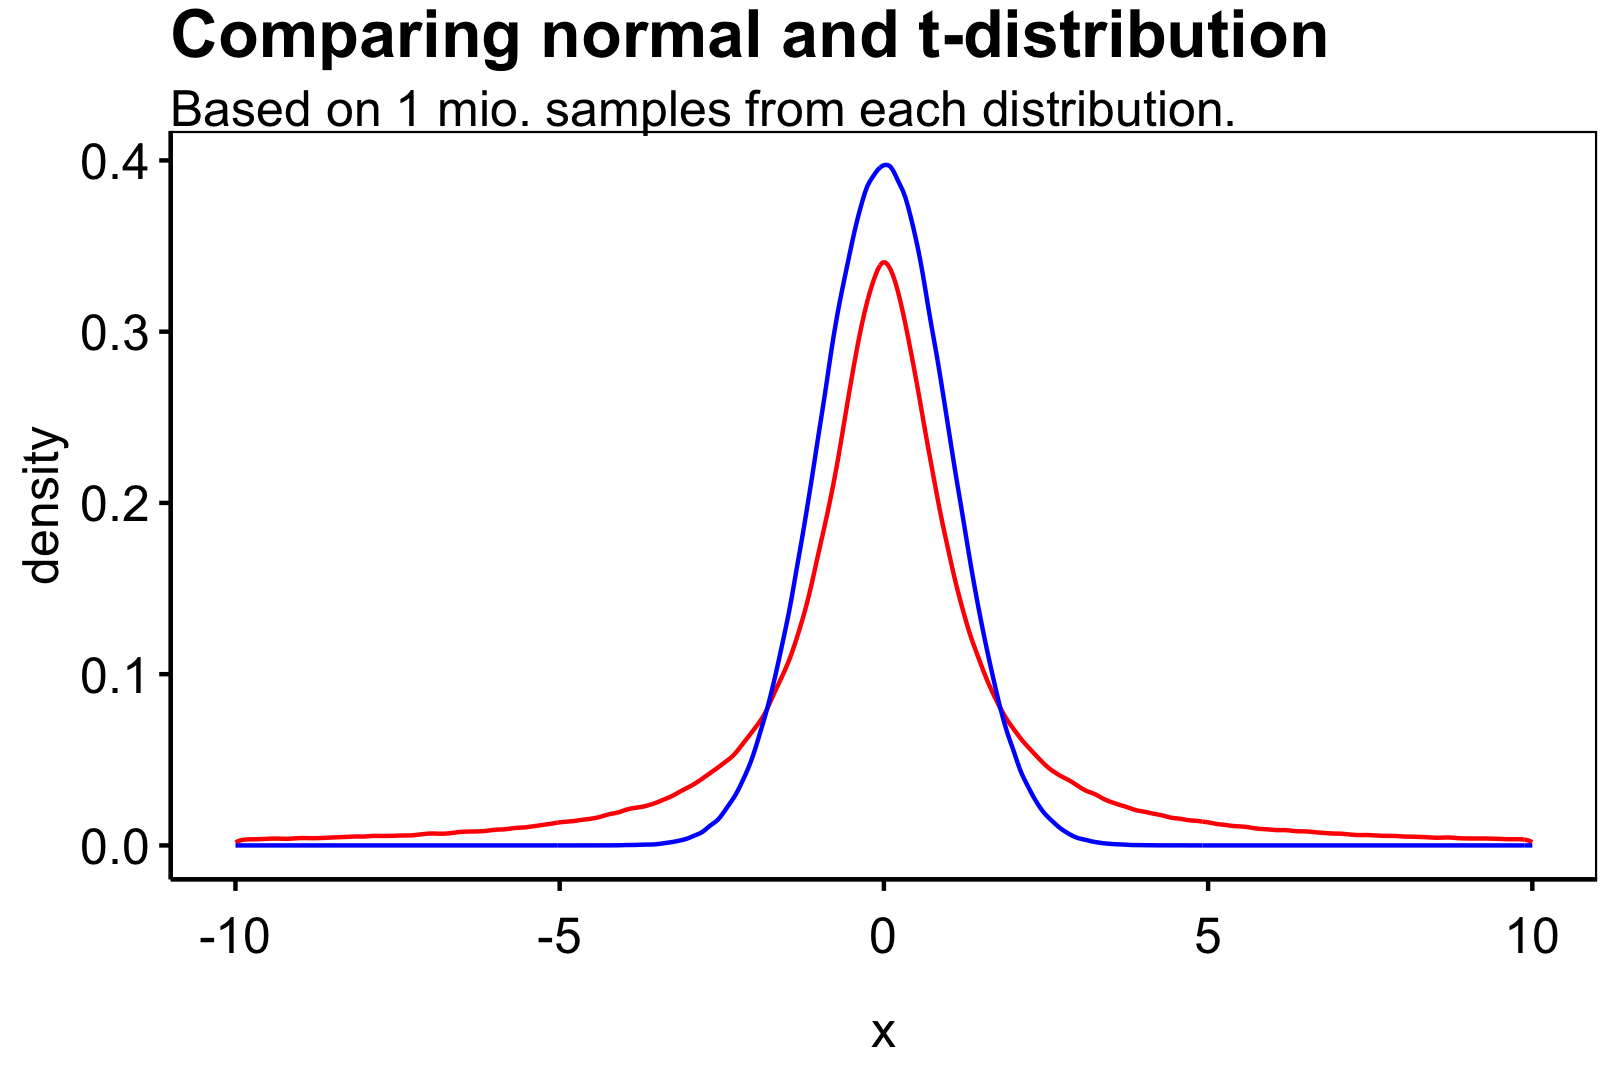
\includegraphics[width=0.48\textwidth]{figures/ML_week1_ex3.png}
  \end{center}
\end{figure}

This gives that for a given sample size the risk will tend to infinity as \(n\) grows to infinity. This in turn explains the large values we see in the risk. We see that for the \(t\)-distribution with one degree of freedom we see the same relation as in the normal case. The median does better in the \(L_1\) loss but worse under the squared loss.

\textbf{Exercise 4.} We want to practise model tuning with the mlr3 package. Go through the following steps:

\begin{enumerate}
\def\labelenumi{\arabic{enumi}.}
\tightlist
\item
  Install and load the relevant ml3 packages: mlr3, mlr3learners, mlr3tuning, mlr3mbo.
\item
  Create a task
\end{enumerate}

\begin{itemize}
\tightlist
\item
  Load the \texttt{mtcars} data (write: \emph{data(mtcars)})
\item
  Use the \texttt{as\_task\_regr} to create a task with \texttt{mpg} as target
\end{itemize}

\begin{enumerate}
\def\labelenumi{\arabic{enumi}.}
\setcounter{enumi}{2}
\tightlist
\item
  Set \texttt{regr.xgboost} as learner with corresponding search space; e.g.,
  \begin{align*}
  eta &= to\_tune(0, 1)\\
  nrounds &= to\_tune(10, 5000)\\
  max\_depth &= to\_tune(1, 20)\\
  colsample\_bytree &= to\_tune(0.1, 1)\\
  subsample &= to\_tune(0.1, 1)
  \end{align*}
\item
  Tune your learner on you task using the \texttt{tune} function with
\end{enumerate}

\begin{itemize}
\tightlist
\item
  Resampling method: 5-fold cross validation
\item
  Measure: squared loss
\item
  Method: \texttt{mbo} or \texttt{random\ search}
\item
  Terminator: 10 evaluations
\end{itemize}

\begin{enumerate}
\def\labelenumi{\arabic{enumi}.}
\setcounter{enumi}{4}
\tightlist
\item
  Fit your learner on the task using the optimal hyper parameters calculated
\end{enumerate}

\textbf{Solution (1).}

We install the required packages.

\textbf{Solution (2).}

We start by loading the data.

We now transform the data into a task.

We may now split out data set into random partions of a training dataset and a testing dataset.

We see that the testing dataset has \(N_1=11\) and the training dataset has \(N_2=21\). We will be training the model on the training dataset. Therefore we start a task on the subset.

\textbf{Solution (3).}

We now initiate a learner.

We can now look at the current configuration of the leaner by looking at the parameter space of the hyperparameter.

As the text says we set som of the parameters to as specific section of the parameter space.

\textbf{Solution (4).}

We tune a regression model using \texttt{mbo} search.

We can consider the the estimates from each subset and the fitted parameters.

\textbf{Solution (5).}

We can now use optimal paramteres in \texttt{instance\$result\_learner\_param\_vals} to create a learner that we may fit to the training data.

We now fit the data.

We can now predict onto the testing data.

Using a diagram we can see. That the model does pretty well. In fact the empirical risk is 6.38.

\begin{figure}[H]
  \begin{center}
    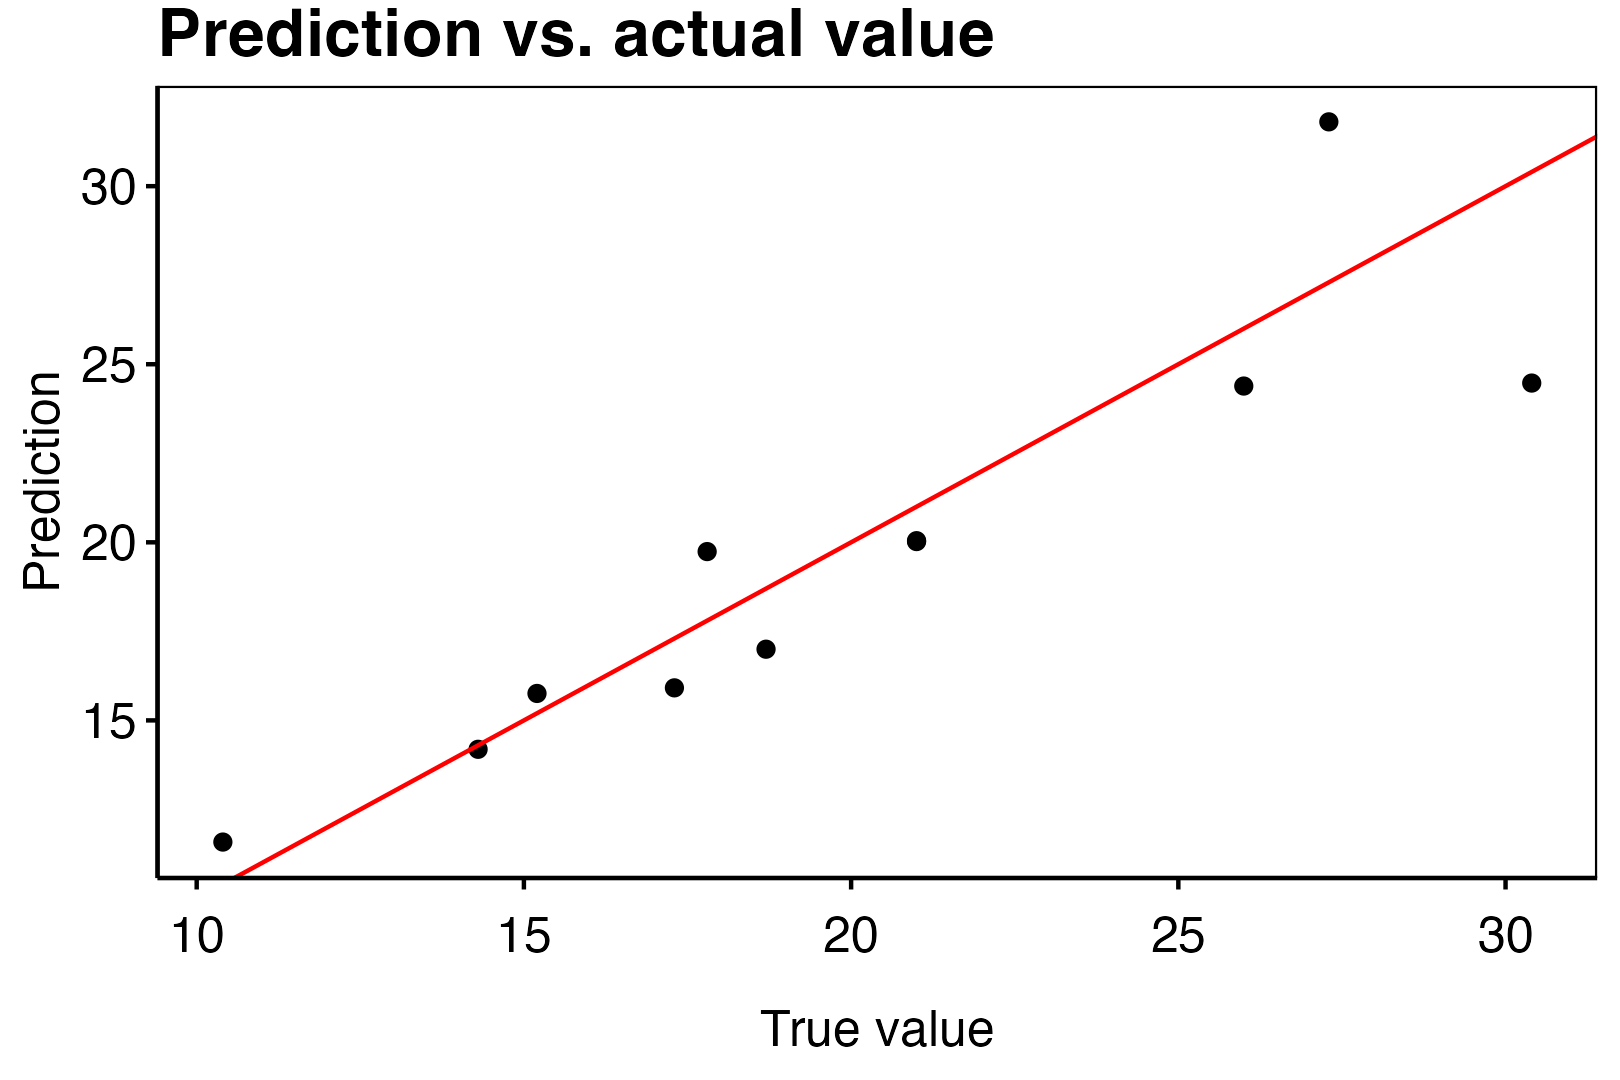
\includegraphics[width=0.48\textwidth]{figures/ML_week1_ex4.png}
  \end{center}
\end{figure}

\hypertarget{week-2-1}{%
\section{Week 2}\label{week-2-1}}

From now on, given sample size \(n\), a dimension \(p\), and a correlation parameter \(0\le \texttt{rho}<1\) we will generate data \(X\) via the following code.

The resulting features will have approximately support on \([−1, 1]\) and will have approximately pairwise correlation of size \(\texttt{rho}\). Given the distribution of \(\varepsilon\) and a regression function \(m\), we then generate data \((X_i,Y_i)_{i=1,...,n}\) via

\[
Y_i=m(X_i)+\varepsilon_i,
\]

where \(\varepsilon_i\) are iid copies of \(\varepsilon\) and \(X_i\) is the \(i\)th row of \(X\).

\textbf{Exercise 1.} We want to try out ordinary least squares regression, lasso, ridge regression and elastic net on some different data generating settings (Model 1--4).

\begin{longtable}[]{@{}
  >{\raggedright\arraybackslash}p{(\columnwidth - 12\tabcolsep) * \real{0.1429}}
  >{\centering\arraybackslash}p{(\columnwidth - 12\tabcolsep) * \real{0.1429}}
  >{\centering\arraybackslash}p{(\columnwidth - 12\tabcolsep) * \real{0.1429}}
  >{\centering\arraybackslash}p{(\columnwidth - 12\tabcolsep) * \real{0.1429}}
  >{\centering\arraybackslash}p{(\columnwidth - 12\tabcolsep) * \real{0.1429}}
  >{\centering\arraybackslash}p{(\columnwidth - 12\tabcolsep) * \real{0.1429}}
  >{\centering\arraybackslash}p{(\columnwidth - 12\tabcolsep) * \real{0.1429}}@{}}
\toprule()
\begin{minipage}[b]{\linewidth}\raggedright
\end{minipage} & \begin{minipage}[b]{\linewidth}\centering
n
\end{minipage} & \begin{minipage}[b]{\linewidth}\centering
p
\end{minipage} & \begin{minipage}[b]{\linewidth}\centering
s
\end{minipage} & \begin{minipage}[b]{\linewidth}\centering
rho
\end{minipage} & \begin{minipage}[b]{\linewidth}\centering
m
\end{minipage} & \begin{minipage}[b]{\linewidth}\centering
\(\varepsilon\)
\end{minipage} \\
\midrule()
\endhead
Model 1 & 1000 & 100 & 5 & 0.3 & \(\sum_{j=1}^s x_j\) & \(\mathcal N(0,1)\) \\
Model 2 & 1000 & 100 & 100 & 0.3 & \(\sum_{j=1}^s x_j\) & \(\mathcal N(0,1)\) \\
Model 3 & 1000 & 100 & 5 & 0.3 & \(\sum_{j=1}^s 0.1x_j\) & \(\mathcal N(0,1)\) \\
Model 4 & 1000 & 100 & 100 & 0.3 & \(\sum_{j=1}^s 0.1x_j\) & \(\mathcal N(0,1)\) \\
\bottomrule()
\end{longtable}

\begin{enumerate}
\def\labelenumi{\alph{enumi}.}
\tightlist
\item
  Given one set of training data for each model tune (i.e.~estimate optimal hyperprameter) via 5-fold cross-validation using a search method and number of evals of your choice. You should now have an estimated optimal hyperparameter for every combination of model and method.
\item
  Generate 100 test sets each of size n for every model and calculate empirical mean and standard deviation of the test error for each method and model using the hyperparameters calculated in (a). Create a table of your results (each missing entry should show hyperparameter: mean(sd)):
\end{enumerate}

\begin{longtable}[]{@{}lcccc@{}}
\toprule()
& Least Squares & Ridge & Lasso & Elastic Net \\
\midrule()
\endhead
Model 1 & \(\cdot\) & \(\cdot\) & \(\cdot\) & \(\cdot\) \\
Model 2 & \(\cdot\) & \(\cdot\) & \(\cdot\) & \(\cdot\) \\
Model 3 & \(\cdot\) & \(\cdot\) & \(\cdot\) & \(\cdot\) \\
Model 4 & \(\cdot\) & \(\cdot\) & \(\cdot\) & \(\cdot\) \\
\bottomrule()
\end{longtable}

\begin{enumerate}
\def\labelenumi{\alph{enumi}.}
\setcounter{enumi}{2}
\tightlist
\item
  Discuss why test error alone might often not be the (only) quantity of interest.
\end{enumerate}

\textbf{Solution (a).}

We start by simulating the data with the seed 1 for the training data and 2 for testing data.

\textbf{Model 1}

We may now estimate under model 1 by setting the parameters and generating the data.

We can estimate the optimal parameters under least squares estimation with the \texttt{lm} function.

We can use \texttt{predict} to see the model prediction vs.~the true values.

\begin{figure}[H]
  \begin{center}
    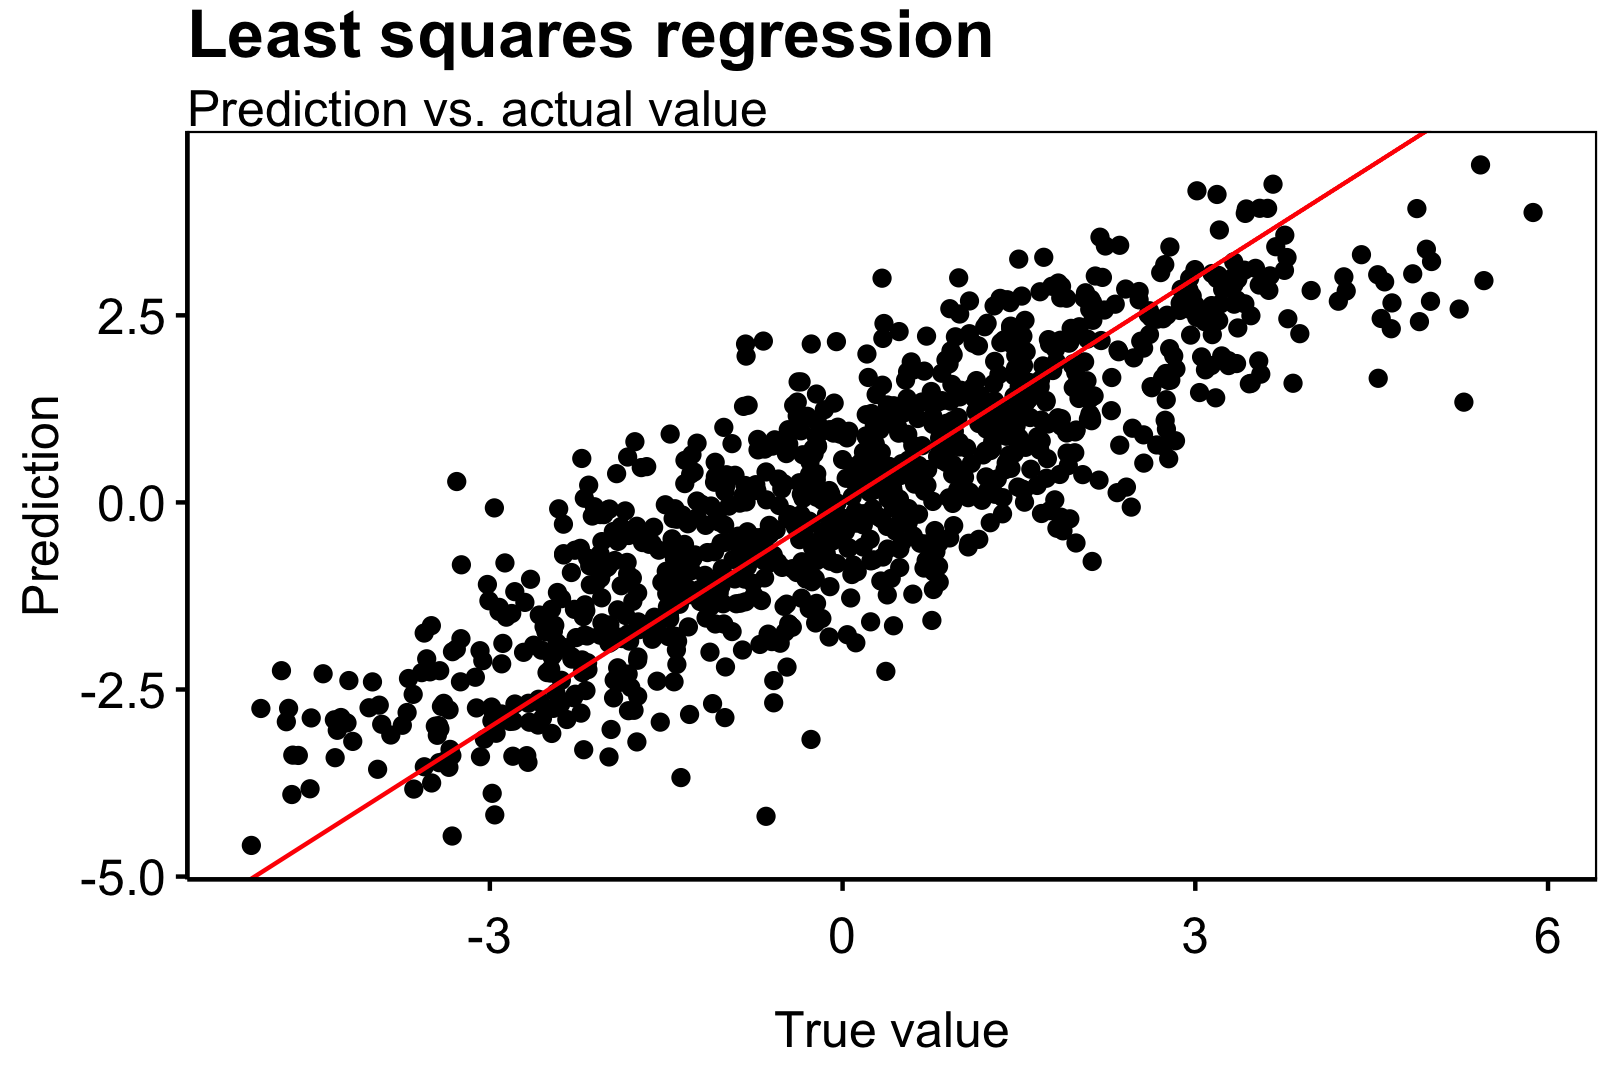
\includegraphics[width=0.48\textwidth]{figures/ML_week2_ex1_01.png}
  \end{center}
\end{figure}

We can also use \texttt{mlr3} to tune optimal hyperparameters for a lasso, ridge and elastic net estimator. We start as usual by slitting the data into training and testing datasets and starting a task.

We can now initiate a leaner. We start by fitting the hyperparameter for the lasso learner.

We use the \texttt{glmnet} as it is an algorithm that solves the minimizing problem

\[
\hat{\beta}_\lambda^{\text {glmnet }} =\underset{\beta \in \mathbb{R}^p}{\arg \min }\left\{\hat{R}_n(\beta)+J_\lambda(\beta)\right\},\hspace{15pt}J_\lambda(\beta)=\lambda \left[\alpha\sum_{j=1}^p\left|\beta_j\right|+\frac{1-\alpha}{2}\sum_{j=1}^p\beta_j^2\right],
\]

One may recall that the lasso estimator is given by

\[
\hat{\beta}_\lambda^{\text {lasso }} =\underset{\beta \in \mathbb{R}^p}{\arg \min }\left\{\hat{R}_n(\beta)+J_\lambda(\beta)\right\},\hspace{15pt}J_\lambda(\beta)=\lambda \sum_{j=1}^p\left|\beta_j\right|,
\]

and so the lasso estimator is a specialcase of the \texttt{glmnet} with \(\alpha=1\). From the above we see that the minimizing algorithm punishes large beta's. The hyperparameter to tune is then \(\lambda\ge 0\) (\texttt{s} is the syntax for \(\lambda\)). Looking at the parameters in the \texttt{learner\_lasso} one can see the entire hyperparameter space.

Let us tune a lasso learner by setting \texttt{alpha\ =\ 1} and tuning \texttt{s\ =\ totune(0,1)} i.e.~searching for \(\lambda \in [0,1]\).

Now that we have tuned the algorithm we can fit the model with the above \(s\) (0.0618).

Lets quickly look at the predictions.

\begin{figure}[H]
  \begin{center}
    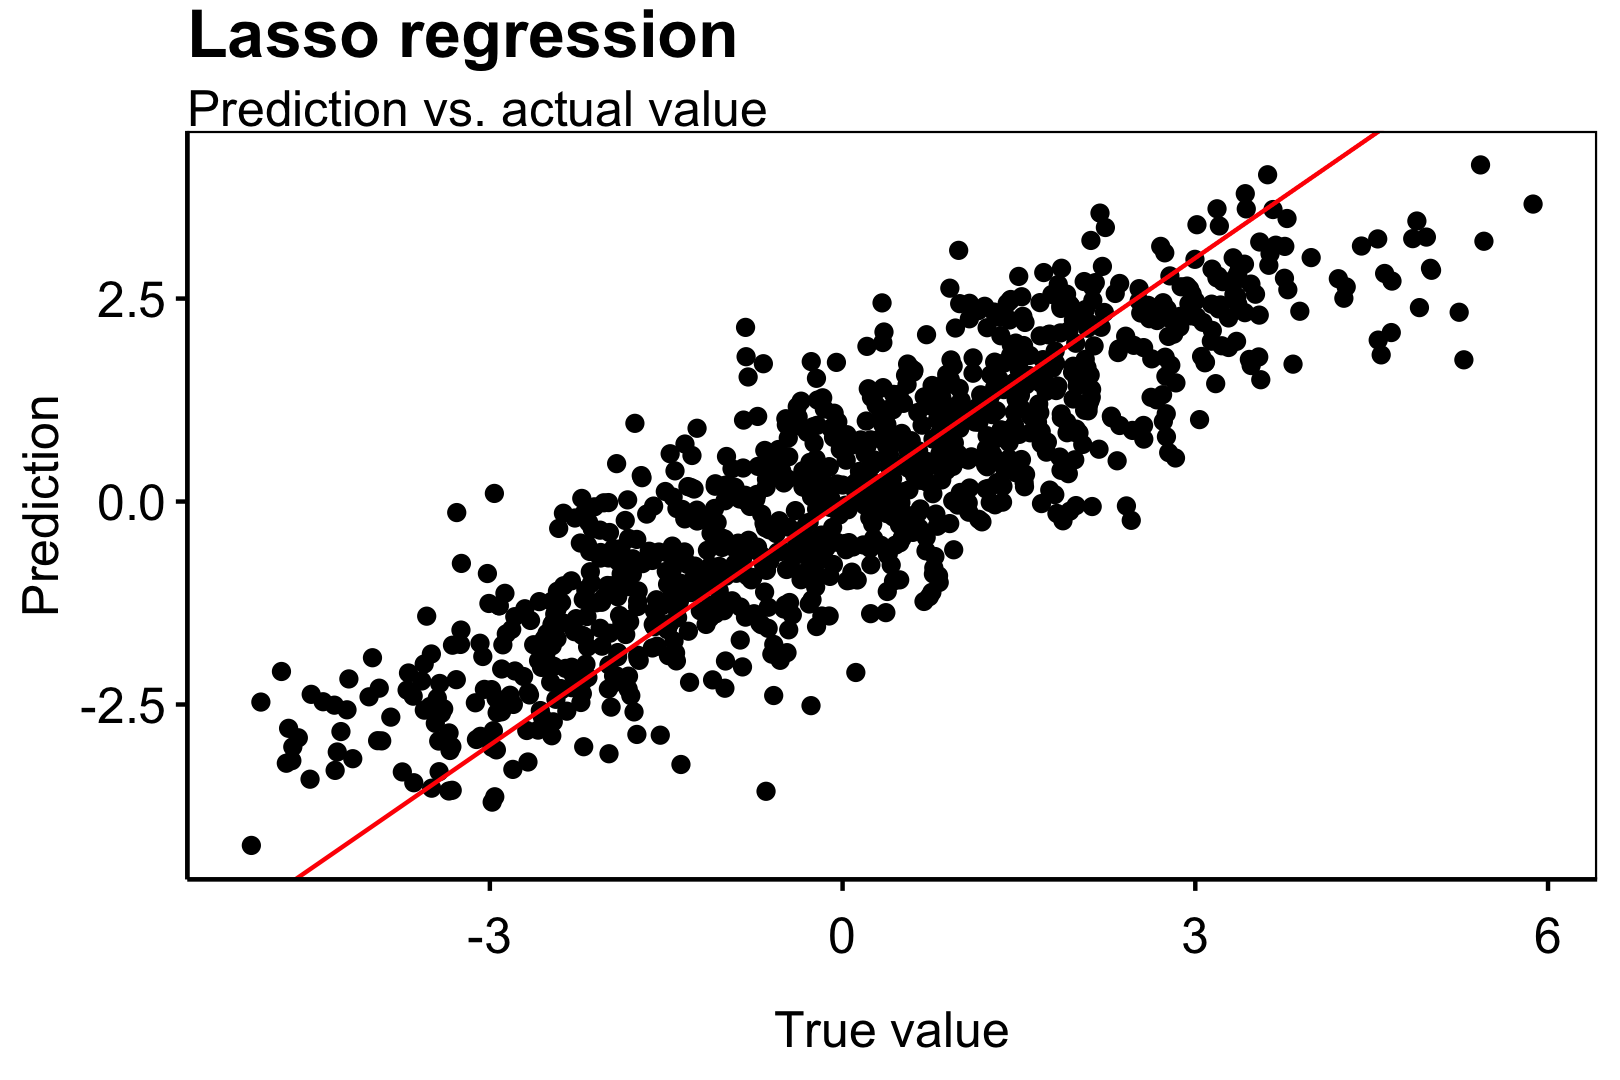
\includegraphics[width=0.48\textwidth]{figures/ML_week2_ex1_02.png}
  \end{center}
\end{figure}

One can get the coefficients of \(\beta\) by predicting the data frame \texttt{I\ =\ diag(1,nrow\ =\ 100)} being the identity.

One can see that the values is close to the true value \(\beta=(1,1,1,1,1,0,...,0)\).

We can now estimate the parameters in ridge regression by setting \(\alpha = 0\) and then getting a scaled version of \(\lambda\).

We fit the model with the above \(s\) (0.22).

Lets quickly look at the predictions.

\begin{figure}[H]
  \begin{center}
    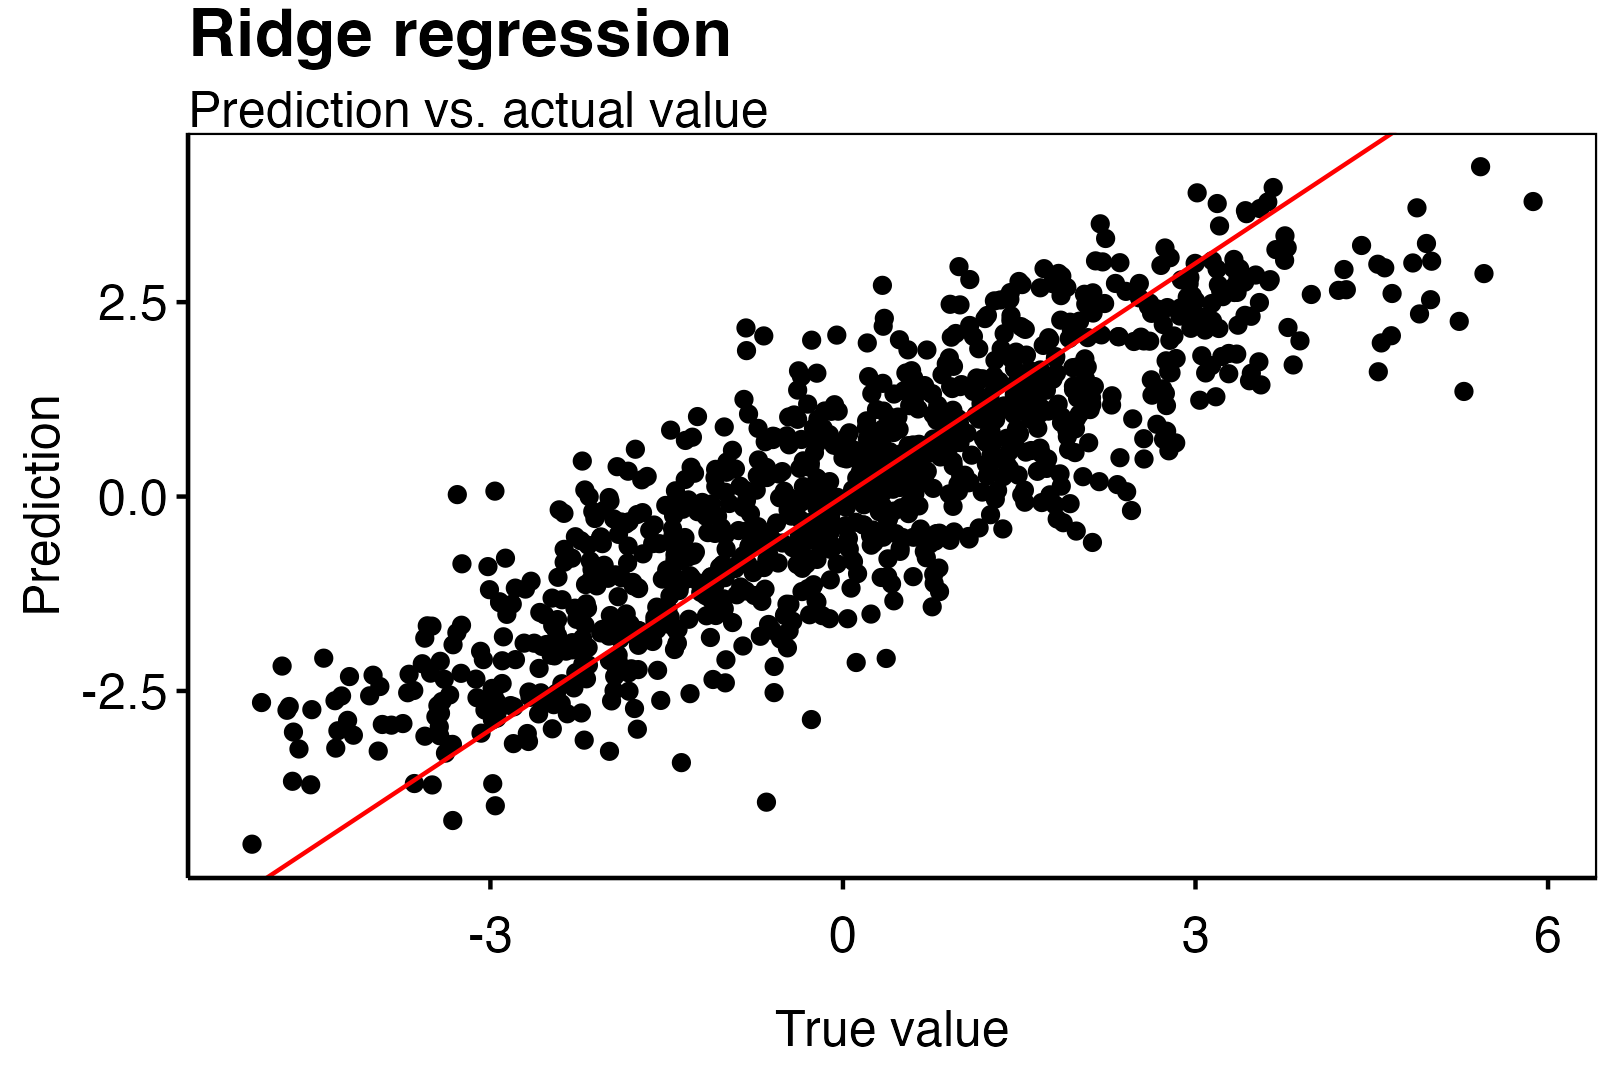
\includegraphics[width=0.48\textwidth]{figures/ML_week2_ex1_03.png}
  \end{center}
\end{figure}

For good measures we calculate the beta's as in lasso.

Finally, let us tune an elastic net.

We fit the model with the above \(s\) (0.0623).

Lets quickly look at the predictions.

\begin{figure}[H]
  \begin{center}
    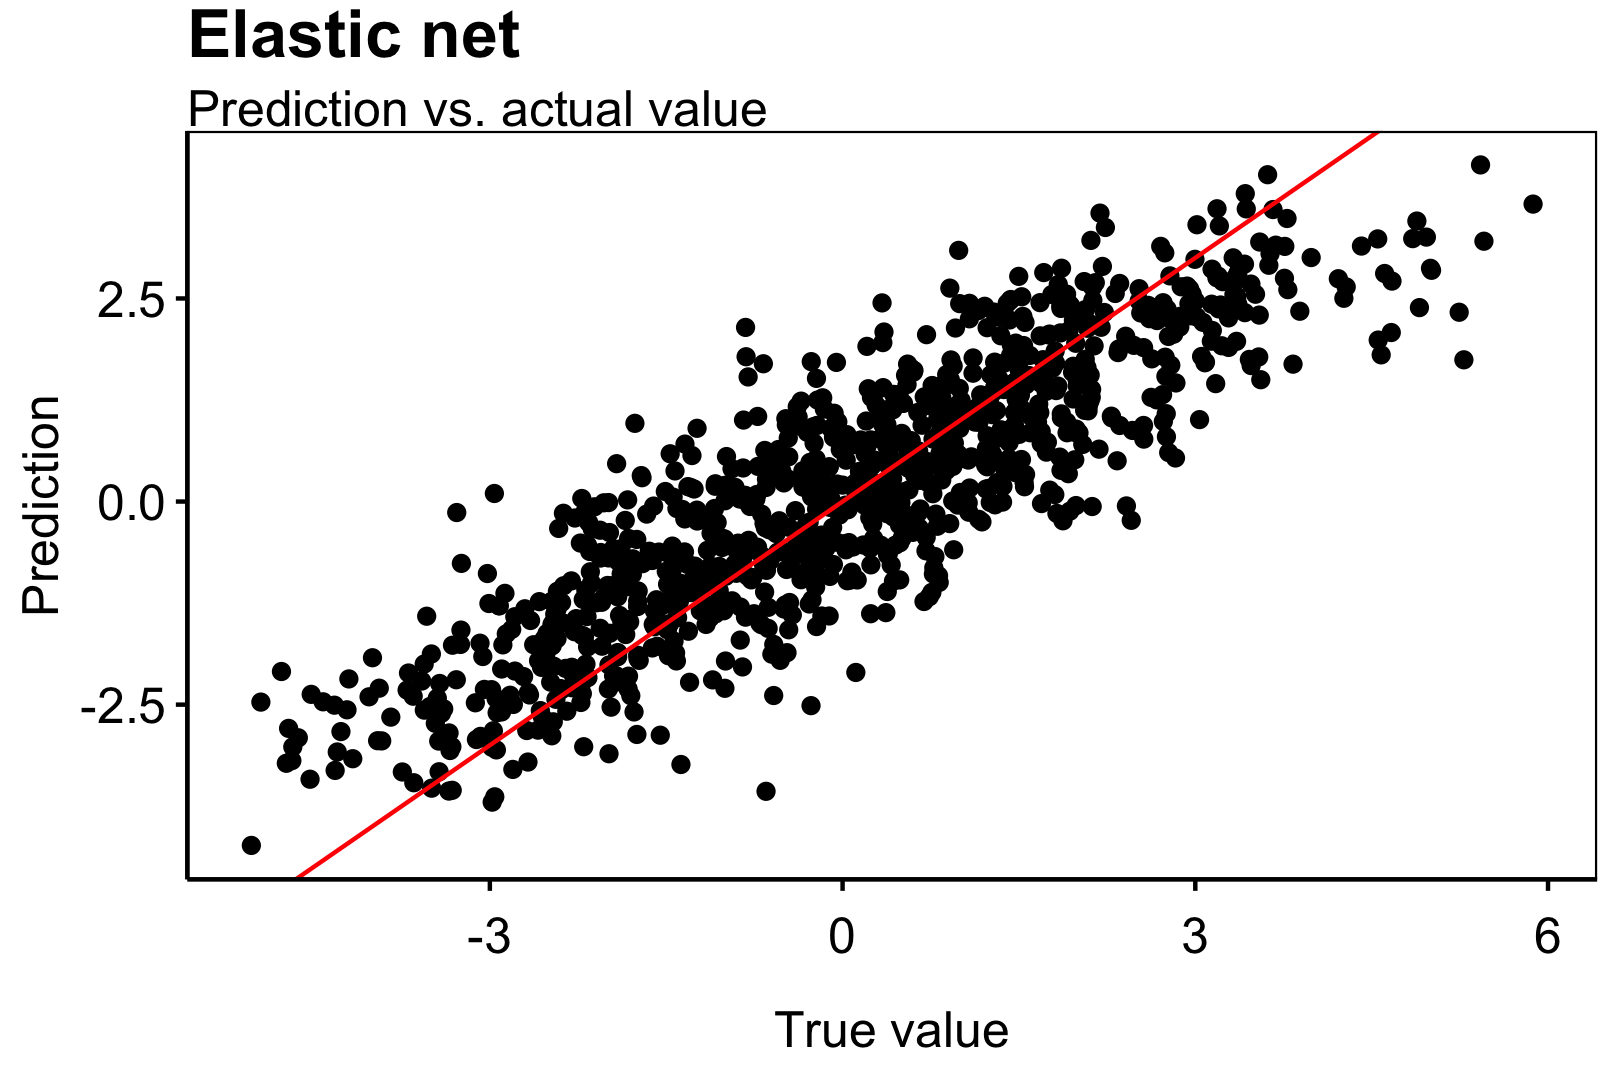
\includegraphics[width=0.48\textwidth]{figures/ML_week2_ex1_04.png}
  \end{center}
\end{figure}

For good measures we calculate the beta's as in lasso.

Let's lastly look at how the different estimators do with respect to the true beta.

\begin{figure}[H]
  \begin{center}
    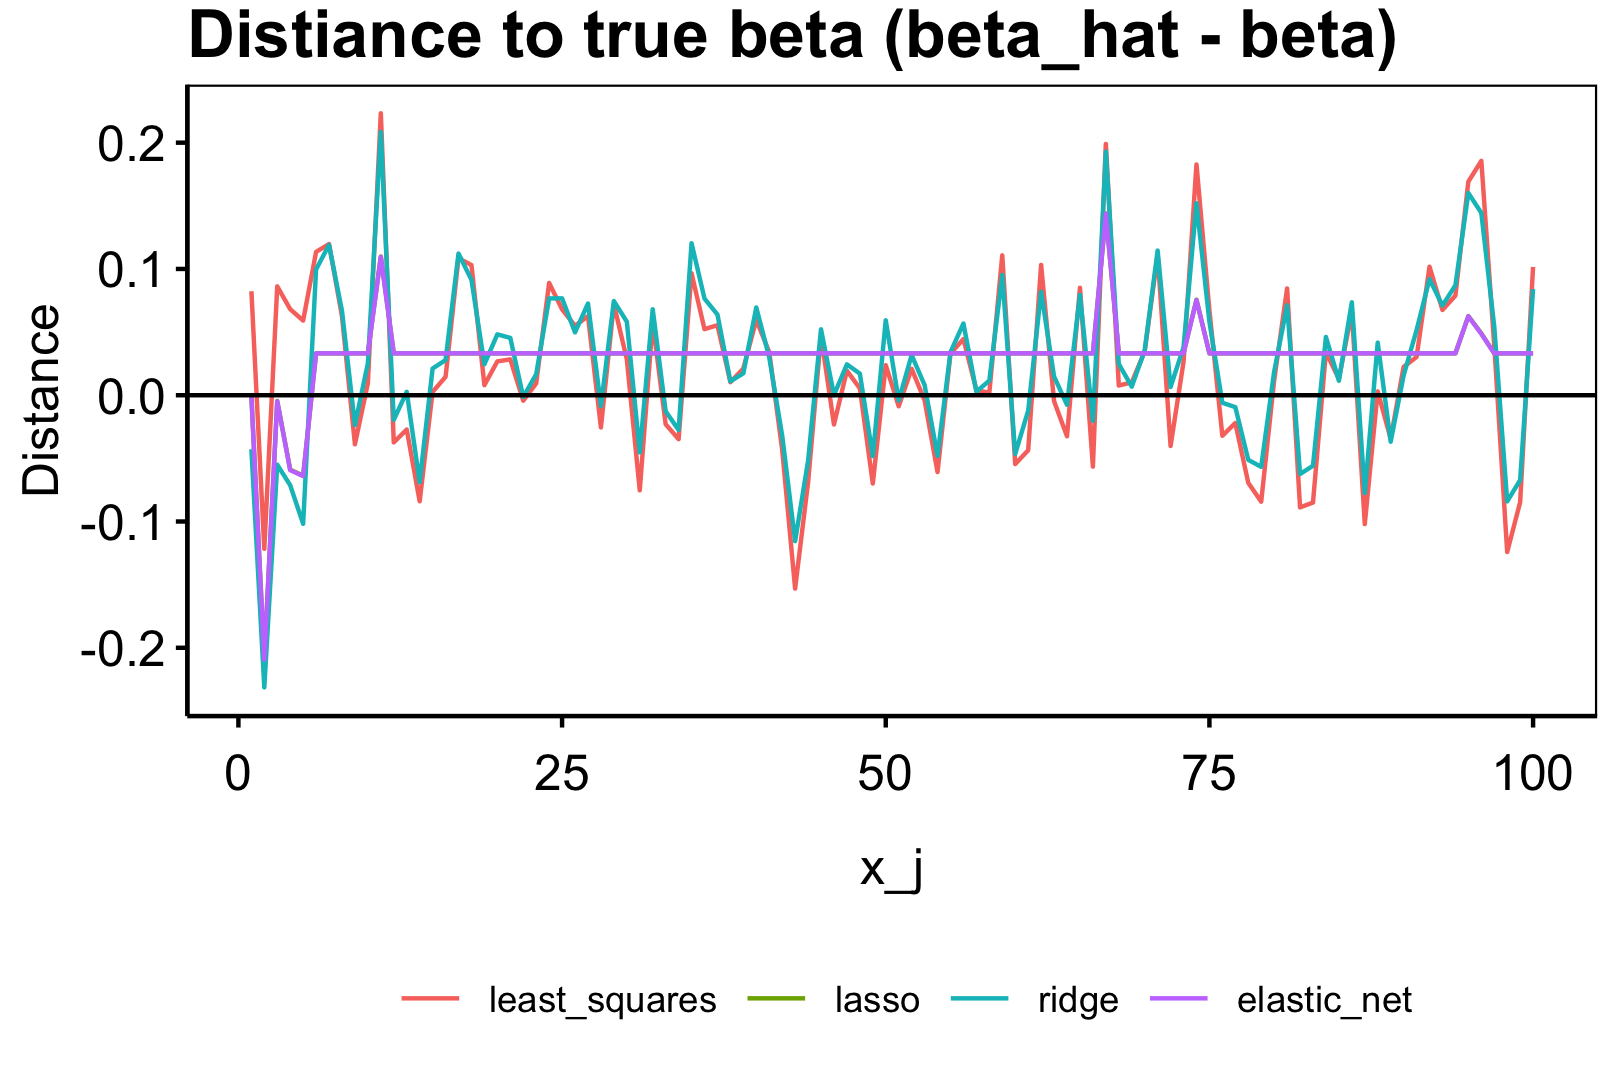
\includegraphics[width=0.48\textwidth]{figures/ML_week2_ex1_05.png}
  \end{center}
\end{figure}

We may now estimate the remaining three models.

\textbf{Model 2-4.} We generate the data and estimate under the model. We define a function that compute the estimators.

Now we simply gather the results.

\textbf{Solution (b).}

We simply generate \(N=100\) test sets and compute the mean squared error for each run, then take the empirical mean and standard deviation of the 100 samples of the empirical mean squared error.

\textbf{Solution (c).}

In general, it is better to have as small of a test error as possible. It it however also important not to overcomplicate the model if not all variables is relevant. Ridge regression does well in the models with fewer explanatory variable \(s\) as it punishes under \(L^2\) distance rather than \(L^1\). This means that ridge does a better job in setting \(\beta_j\approx 0\) for \(j> s\).

\hypertarget{week-3-1}{%
\section{Week 3}\label{week-3-1}}

\textbf{Exercise 1.} Random forests are known for their computational speed and can be used in settings with thousands of features. Here we discuss how it is usually decided where to split a node. Assume we have n observations at a node, and want to find the optimal split. The \texttt{mtry} provides us with a list of possible features to split. Fix one feature and assume that observations in that node are sorted according to the value of that feature. In the current node the squared loss is

\[
Q=\sum_{i=1}^n(x_i-\overline x)^2=\sum_{i=1}^nx_i^2-n\overline{x}^2.
\]

Define

\[
Q_L(k)=\sum_{i=1}^k(x_i-\overline{x}_k^+)^2,\qquad Q_R(k)=\sum_{i=k+1}^n(x_i-\overline{x}_k^-)^2
\]

where

\[
\overline{x}_k^+=\frac{1}{k}\sum_{i=1}^kx_i\quad \text{and}\quad \overline{x}_k^-=\frac{1}{n-k}\sum_{i=k+1}^nx_i.
\]

The node is split at that \(k\) that minimizes \(Q_L(k)+Q_R(k)\). Discuss how the optimal \(k\) can be found more efficiently than calculating for every \(k\) \(Q_L(k)+Q_R(k)\) from scratch.

\textbf{Solution.}

\textbf{Exercise 2.} We extend the framework from previous week and now also consider classification tasks. When considering a classification task, the only change in the data generation compared to the regression setting is that we generate the response \(Y\) via

\[
Y=\frac{\text{sign}(m(X_i)+\varepsilon_i)+1}{2}.
\]

Try out least squares regression and classification with least squares and binary loss. As learners, we will work with linear regression/logistic regression (with e.g.~elastic net penalization), generalized additive models from the \texttt{mgcv} package and random forest via the \texttt{ranger} package. Part of the task is to figure out how to optimize the (penalty) parameters to be successful in the sparse settings as given below. We will consider the following models.

\begin{longtable}[]{@{}
  >{\raggedright\arraybackslash}p{(\columnwidth - 12\tabcolsep) * \real{0.1429}}
  >{\centering\arraybackslash}p{(\columnwidth - 12\tabcolsep) * \real{0.1429}}
  >{\centering\arraybackslash}p{(\columnwidth - 12\tabcolsep) * \real{0.1429}}
  >{\centering\arraybackslash}p{(\columnwidth - 12\tabcolsep) * \real{0.1429}}
  >{\centering\arraybackslash}p{(\columnwidth - 12\tabcolsep) * \real{0.1429}}
  >{\centering\arraybackslash}p{(\columnwidth - 12\tabcolsep) * \real{0.1429}}
  >{\centering\arraybackslash}p{(\columnwidth - 12\tabcolsep) * \real{0.1429}}@{}}
\toprule()
\begin{minipage}[b]{\linewidth}\raggedright
\end{minipage} & \begin{minipage}[b]{\linewidth}\centering
n
\end{minipage} & \begin{minipage}[b]{\linewidth}\centering
p
\end{minipage} & \begin{minipage}[b]{\linewidth}\centering
s
\end{minipage} & \begin{minipage}[b]{\linewidth}\centering
rho
\end{minipage} & \begin{minipage}[b]{\linewidth}\centering
m
\end{minipage} & \begin{minipage}[b]{\linewidth}\centering
\(\varepsilon\)
\end{minipage} \\
\midrule()
\endhead
Model 1 & 1000 & 100 & 5 & 0.3 & \(\sum_{j=1}^s x_j\) & \(\mathcal N(0,1)\) \\
Model 3 & 1000 & 100 & 5 & 0.3 & \(\sum_{j=1}^s 0.1x_j\) & \(\mathcal N(0,1)\) \\
Model 5 & 1000 & 100 & 5 & 0.3 & \(\sum_{j=1}^s m_j(x_j)\) & \(\mathcal N(0,1)\) \\
Model 6 & 1000 & 100 & 5 & 0.3 & \(\sum_{j=1}^s m_j(x_j)+\sum_{j=1}^{s-1} m_j(x_jx_{j+1})\) & \(\mathcal N(0,1)\) \\
\bottomrule()
\end{longtable}

Here \(m_j(x_j)=(-1)^j2\sin(\pi x_j)\)

\begin{enumerate}
\def\labelenumi{\alph{enumi}.}
\tightlist
\item
  For each of the three settings (regression: squared loss, classification: squared loss, classification: binary loss), given one set of training data for each model tune (i.e.~estimate optimal hyperprameter) via 5-fold cross-validation using a search method and number of evals of your choice. You should now have an estimated optimal hyperparameter for every combination of setting, model and learner.
\item
  Generate 100 test sets each of size n for every setting, model and learner and calculate empirical mean and standard deviation of the test error for each setting, model and learner using the hyperparameters calculated in (a). Create three tables ofor your results (each missing entry should show hyperparameter: mean(sd)):
\end{enumerate}

\begin{longtable}[]{@{}lcccc@{}}
\toprule()
& Linear model & glm & Random forest & \\
\midrule()
\endhead
Model 1 & \(\cdot\) & \(\cdot\) & \(\cdot\) & \\
Model 3 & \(\cdot\) & \(\cdot\) & \(\cdot\) & \\
Model 5 & \(\cdot\) & \(\cdot\) & \(\cdot\) & \\
Model 6 & \(\cdot\) & \(\cdot\) & \(\cdot\) & \\
\bottomrule()
\end{longtable}

\textbf{Solution (a).}

\textbf{Solution (b).}

\hypertarget{topics-in-life-insurance}{%
\chapter{Topics in Life Insurance}\label{topics-in-life-insurance}}

\hypertarget{computing-moments-of-reserve-in-timehomogeneous-case}{%
\section{Computing moments of reserve in timehomogeneous case}\label{computing-moments-of-reserve-in-timehomogeneous-case}}

In this exercise we consider a time-homogeneous Markov jump process \(X\) on the state-space \(E=\{1,...,5\}\) defined as such

\begin{enumerate}
\def\labelenumi{\arabic{enumi}.}
\tightlist
\item
  Active,
\item
  Inactive,
\item
  Unemployed,
\item
  Active after unemployment,
\item
  Dead.
\end{enumerate}

The associated intensity matrix \(\mathbf \Lambda\) is

\[
\mathbf\Lambda(x)=\mathbf \Lambda=
\begin{bmatrix}
-0.7 & 0.1 & 0.1&    &0.5 \\
 &-0.5 &  &  & 0.5 \\
 & 0.1& -0.7 & 0.1 & 0.5\\
 & 0.1 & & -0.6 & 0.5\\
 &  &  &  & \\
\end{bmatrix}.
\]

Where all zero entries are left blank. We consider the insurance contract that,

\begin{itemize}
\tightlist
\item
  Insured pays \(\rho\) as long as he is alive,
\item
  Insured recieve 1 while unemployed or inactive and
\item
  Insured receive 2 if he becomes inactive. If he is active just before the jump this only happends with probability \(1/2\).
\end{itemize}

The contract expires at time \(T=1\) and we assume \(X(0)=1\). We want to compute the equivalence premium for a constant interest rate \(r=0\).

\begin{enumerate}
\def\labelenumi{\alph{enumi}.}
\tightlist
\item
  Determine \(\mathbf B(t)\) and \(b\).
\item
  Decompose \(\mathbf \Lambda\) into \(\mathbf \Lambda=\mathbf \Lambda^0+\mathbf \Lambda^1\) and compute the rewards \(\mathbf R\).
\item
  Compute the reserve at time \(t=0\) for \(\rho = -1\).
\item
  Compute the equivalence premium \(\hat\rho\) and check that \(\mathbf V(0;X(0)=0)=0\).
\item
  Compute the contributions \(\mathbf C_r^{(2)}\) and use this to compute the second moment \(\mathbf V^{(2)}(0;X(0)=0)\).
\end{enumerate}

\textbf{Solution (a).}

The matrix \(\mathbf B=\left\{b_{ij}\right\}_{i,j\in E}\) is given by \(b_{ij}=2\) if \(j=2\) and \(i\in \{1,3,4\}\) i.e.

\[
\mathbf B=
\begin{bmatrix}
0 & 2 &0 &0 & 0 \\
0 & 0 &0 &0 & 0 \\
0 & 2 &0 &0 & 0 \\
0 & 2 &0 &0 & 0 \\
0 & 0 &0 &0 & 0 \\
\end{bmatrix}.
\]

The continuous payment rate is

\[
b=\begin{pmatrix}
\rho\\
1\\
1\\
\rho\\
0
\end{pmatrix}.
\]

We implement this i R using.

\textbf{Solution (b).}

The \(\mathbf \Lambda\) is decomposed by setting \((\lambda^1_{12},\lambda^1_{32},\lambda^1_{42})=(\lambda_{12}/2,\lambda_{32},\lambda_{42}/2)\) and the rest to 0 since the payment when transitioning from 1 or 4 only happens with probabiltiy \(1/2\). The reward matrix is simply given by \(\mathbf R=\mathbf \Lambda^1 \bullet \mathbf B + \Delta b\) i.e.

\[
\mathbf R = 
\begin{bmatrix}
\rho & 2\lambda_{12}^1 &0 &0 & 0 \\
0 & 1 &0 &0 & 0 \\
0 & 2\lambda_{32}^1 &1 &0 & 0 \\
0 & 2\lambda_{42}^1 &0 &\rho & 0 \\
0 & 0 &0 &0 & 0 \\
\end{bmatrix}.
\]

We implement in R.

\textbf{Solution (c).}

We compute the reserve by using the following

\[
\prod_t^T\left(\mathbf I+\begin{pmatrix}
\mathbf \Lambda-\Delta(r) & \mathbf R\\
\mathbf 0 & \mathbf \Lambda
\end{pmatrix}\ dx\right)=
\begin{pmatrix}
e^{-\int_t^Tr\ du}\mathbf P(t,T) & \mathbf V(t,T)\\
\mathbf 0 & \mathbf P(t,T)
\end{pmatrix}.
\]

We then compute

\[
V(t,T)=e_1^\top \mathbf V(t,T)e.
\]

\textbf{Solution (d).}

The equivalence premium is computed by

\[
\hat \rho = \left.-\frac{e_1^\top \mathbf V(t,T)e}{e_1^\top \mathbf V'(t,T)e}\right\vert_{\rho=0},
\]

with \(\mathbf V'(t,T)\) defined by

\[
\prod_t^T\left(\mathbf I+\begin{pmatrix}
\mathbf \Lambda-\Delta(r) &\frac{\partial}{\partial \rho} \mathbf R(\rho)\\
\mathbf 0 & \mathbf \Lambda
\end{pmatrix}\ dx\right)=
\begin{pmatrix}
e^{-\int_t^Tr\ du}\mathbf P(t,T) & \mathbf V'(t,T)\\
\mathbf 0 & \mathbf P(t,T)
\end{pmatrix}.
\]

We compute

Let us see if the reserve is zero as expected.

\textbf{Solution (e).}

We have that

\[
\mathbf C_r^{(k)}=\frac{1}{k!}\mathbf\Lambda^1\bullet \mathbf B^{\bullet k}
\]

and
\begin{align*}
\prod_t^T&\left(\mathbf I+\begin{pmatrix}
\mathbf \Lambda-k\Delta(r) & \mathbf R & \mathbf C_r^{(2)} & \cdots & \mathbf C_r^{(k)}\\
\mathbf 0 & \mathbf \Lambda - (k-1)\Delta(r) & \mathbf R & \cdots & \mathbf C_r^{(k-1)}\\
\vdots & \vdots & \vdots & \ddots & \vdots \\
\mathbf 0 & \mathbf 0 & \mathbf 0 & \cdots & \mathbf \Lambda
\end{pmatrix}\ dx\right)\\
&=
\begin{pmatrix}
* & * & * & \cdots & \mathbf V_r^{(k)}(t,T)\\
* & * & * & \cdots & \mathbf V_r^{(k-1)}(t,T)\\
\vdots & \vdots & \vdots & \ddots & \vdots \\
* & * &* & \cdots &  \mathbf P(t,T)
\end{pmatrix}.
\end{align*}
Where

\[
\mathbf V_r^{(k)}(t,T)=\frac{1}{k!}\mathbf V^{(k)}(t,T).
\]

We therefore implement a Toeplizs block matrix function that for matrices \(\mathbf M_1,...,\mathbf M_k\) generates the matrix

\[
\mathbf M=\begin{pmatrix}
\mathbf M_1 & \mathbf M_2 & \mathbf M_3 &\cdots & \mathbf M_k\\
\mathbf 0 & \mathbf M_1 & \mathbf M_2 & \cdots & \mathbf M_{k-1}\\
\mathbf 0 & \mathbf 0 & \mathbf M_1 & \cdots & \mathbf M_{k-2}\\
\vdots & \vdots & \vdots & \ddots & \vdots\\
\mathbf 0 & \mathbf 0 & \mathbf 0 & \cdots & \mathbf M_1
\end{pmatrix}
\]

This is done in the \texttt{bToeplitz}

We can then compute the second moment.

We can then see that the variance is 0.27.

\newpage

\printindex

  \bibliography{book.bib,packages.bib}

\end{document}
